\documentclass[final,5p,times,twocolumn,authoryear]{elsarticle} %review=doublespace preprint=single 5p=2 column
%%% Begin My package additions %%%%%%%%%%%%%%%%%%%
\usepackage[hyphens]{url}

  \journal{Atmospheric Research} % Sets Journal name


\usepackage{lineno} % add
\providecommand{\tightlist}{%
  \setlength{\itemsep}{0pt}\setlength{\parskip}{0pt}}

\usepackage{graphicx}
\usepackage{booktabs} % book-quality tables
%%%%%%%%%%%%%%%% end my additions to header

\usepackage[T1]{fontenc}
\usepackage{lmodern}
\usepackage{amssymb,amsmath}
\usepackage{ifxetex,ifluatex}
\usepackage{fixltx2e} % provides \textsubscript
% use upquote if available, for straight quotes in verbatim environments
\IfFileExists{upquote.sty}{\usepackage{upquote}}{}
\ifnum 0\ifxetex 1\fi\ifluatex 1\fi=0 % if pdftex
  \usepackage[utf8]{inputenc}
\else % if luatex or xelatex
  \usepackage{fontspec}
  \ifxetex
    \usepackage{xltxtra,xunicode}
  \fi
  \defaultfontfeatures{Mapping=tex-text,Scale=MatchLowercase}
  \newcommand{\euro}{€}
\fi
% use microtype if available
\IfFileExists{microtype.sty}{\usepackage{microtype}}{}
\bibliographystyle{elsarticle-harv}
\usepackage{longtable}
\usepackage{graphicx}
\ifxetex
  \usepackage[setpagesize=false, % page size defined by xetex
              unicode=false, % unicode breaks when used with xetex
              xetex]{hyperref}
\else
  \usepackage[unicode=true]{hyperref}
\fi
\hypersetup{breaklinks=true,
            bookmarks=true,
            pdfauthor={},
            pdftitle={Hourly Assimilation of Different Sources of Observations Including Satellite Radiances in a Mesoscale Convective System Case During RELAMPAGO. Part I: Impact on the Analysis},
            colorlinks=false,
            urlcolor=blue,
            linkcolor=magenta,
            pdfborder={0 0 0}}
\urlstyle{same}  % don't use monospace font for urls

\setcounter{secnumdepth}{5}
% Pandoc toggle for numbering sections (defaults to be off)

% Pandoc citation processing

% Pandoc header
\usepackage{booktabs}
\usepackage{longtable}
\usepackage{array}
\usepackage{multirow}
\usepackage{wrapfig}
\usepackage{float}
\usepackage{colortbl}
\usepackage{pdflscape}
\usepackage{tabu}
\usepackage{threeparttable}
\usepackage{threeparttablex}
\usepackage[normalem]{ulem}
\usepackage{makecell}
\usepackage{xcolor}



\begin{document}
\begin{frontmatter}

  \title{Hourly Assimilation of Different Sources of Observations Including Satellite Radiances in a Mesoscale Convective System Case During RELAMPAGO. Part I: Impact on the Analysis}
    \author[UBA,CIMA,CNRS]{Paola Belén Corrales\corref{1}}
   \ead{paola.corrales@cima.fcen.uba.ar} 
    \author[UBA,CIMA,CNRS]{Victoria Galligani}
  
    \author[UBA,CIMA,CNRS]{Juan Ruiz}
  
    \author[INPE]{Luiz Sapucci}
  
    \author[SMN,CONICET]{María Eugenia Dillon}
  
    \author[SMN,CONICET,CNRS]{Yanina García Skabar}
  
    \author[SMN]{Maximiliano Sacco}
  
    \author[NCAR]{Craig S. Schwartz}
  
      \address[UBA]{Universidad de Buenos Aires, Facultad de Ciencias Exactas y Naturales, Departamento de Ciencias de la Atmósfera y los Océanos. Buenos Aires, Argentina.}
    \address[CIMA]{CONICET -- Universidad de Buenos Aires. Centro de Investigaciones del Mar y la Atmósfera (CIMA). Buenos Aires, Argentina.}
    \address[CNRS]{CNRS -- IRD -- CONICET -- UBA. Instituto Franco-Argentino para el Estudio del Clima y sus Impactos (IRL 3351 IFAECI). Buenos Aires, Argentina.}
    \address[SMN]{Servicio Meteorológico Nacional de Argentina.}
    \address[CONICET]{CONICET (Consejo Nacional de Investigaciones Científicas y Técnicas).}
    \address[INPE]{National Institute for Space Research, Brazil, Center for Weather Forecasting and Climate Studies.}
    \address[NCAR]{National Center for Atmospheric Research, Boulder, Colorado.}
      \cortext[1]{Corresponding Author}
  
  \begin{abstract}
  In this paper we evaluate the impact of assimilating high-resolution surface networks and satellite observations using the WRF-GSI-LETKF. We conducted a case study corresponding to a huge mesoscale convective system (MCS) developed over central and north-eastern Argentina during November 22, 2018. The accumulated precipitation associated with this MCS was quite high, exceeding 200 mm over northern Argentina and Paraguay. This MCS developed during the Intense Observing Period (IOP) of the RELAMPAGO field campaign during November 2018.
  
  We used the GSI-4DLETKF data assimilation package to produce analyses assimilating observations every hour with 10-km horizontal grid spacing and a 60-members ensemble initialized from the deterministic GFS run adding random perturbations with climatological covariance. A multiphysics approach is also used to represent model errors, using different physics configurations (a combination of PBL and convection parameterizations). We conducted four assimilation experiments using different sets of observations: CONV, consisting of conventional observations from NCEP's prepBUFR files, AUT combining CONV and dense automatic surface weather station networks, SATWND, combining AUT with satellite-derived winds and RAD, including SATWND and satellite radiances from different microwave and infrared sensors (AMSU, HIRS, MHS, ATMS, AIRS, and IASI). We found that the assimilation of observations with high temporal and spatial frequency generate an important impact on the PBL, primarily on the precipitable water content, that leads to the development of deep convection and heavy precipitation closer to the observed in this case study. The assimilation of radiance observations produces a better development of the convection mainly during the mature state of the MCS leading to an increase in the accumulated precipitation.
  \end{abstract}
   \begin{keyword} Regional Data Assimilation, Surface Obsevations, Satellite Observations\end{keyword}
 \end{frontmatter}

\hypertarget{introduction}{%
\section{Introduction}\label{introduction}}

Severe weather events cause significant human and material losses around the world. A large number of these phenomena are associated with the occurrence of deep moist convection including tornadoes, intense wind gusts, extreme precipitation in short time periods, large hail, and lightning.
Southern South America has been shown to have the highest frequency of favorable conditions for high-impact meteorological events (Brooks et al., 2003) and the highest occurrence of large hail events (Cecil and Blankenship, 2012).
This is also confirmed by observational evidence and high impact weather reports (Matsudo et al., 2015; Rasmussen et al., 2014).

Forecasting mesoscale meteorological phenomena and particularly deep moist convection is a scientific and technological challenge due to several factors.
On the one hand, mesoscale phenomena have limited predictability, while on the other hand, there is great difficulty in diagnosing the state of the atmosphere at small spatial and short temporal scales (for example from 1 to 10 kilometers and in the order of minutes).
To solve this problem, data assimilation (DA) at the mesoscale is a topic that has gained increasing interest since it can provide appropriate initial conditions for the initialization of high-resolution forecasts (Sun et al., 2014).

DA methods can successfully be implemented by using observations with sufficient temporal and spatial resolution to characterize mesoscale atmospheric circulations.
However, surface observations, which directly measure the atmospheric state, have limited availability in South America.
Other types of observations are being assimilated with relatively high spatial and temporal resolution, such as satellite radiance observations or retrieval products.
Radiance observations are indirect measurements and are more difficult to incorporate into DA systems as they require complex forward models.

The assimilation of conventional observations from surface stations has an important role in improving the initial conditions that lead to better forecasts.
For example, Ha and Snyder (2014) showed that the assimilation of temperature and dew point temperature systematically improved the structure of the simulated planetary boundary layer that subsequently resulted in a better precipitation forecast over the U.S.

Given the sparsity of the local conventional observing network, it is important to explore the potential benefits of including additional sources of observations at a regional scale.
Previous work has shown a positive impact at incorporating temperature and humidity profiles derived from the multispectral infrared sensors (i.e.~AIRS and IASI) in a regional domain application.
Miyoshi and Kunii (2012) assimilated observations, atmospheric temperature, and humidity profile data from the AIRS and found improvement on the tracking of two typhoons.
Dillon et al. (2019) also assimilated retrievals from the AIRS sensor and reported improvements on the thermodynamic variables and the regional circulation.
Moreover, Bao et al. (2015) studied the impact on temperature and humidity forecast over the western USA while assimilating microwave and infrared radiance data and found a reduction in the temperature bias at low and mid-levels as a result of the microwave observations but an opposite effect for infrared data. Recently Zhu et al. (2019) studied the impact of assimilating satellite radiance data within a frequently updated regional system and showed an improvement for all variables, in particular for relative humidity at upper levels.
Satellite-derived winds from water vapor channels and cloud drift motion vectors also have an overall positive impact on analysis and short-range forecasts (Gao et al., 2015).

Having analyses with higher temporal resolution than those available from global forecasting systems (e.g.~at hourly or sub-hourly) and using an increased number of regional observations that are not assimilated in global DA systems are some of the advantages of regional DA.
Previous work has shown promising results on mesoscale DA in the region using different approaches such as LETKF; (Dillon et al., n.d., 2016) and 3D-Var (gustavo Goncalves de Goncalves et al., 2015).
In particular, the use of ensemble-based methods has shown great potential for data assimilation in these scales, as they are able to characterize the flow-dependent evolution of the background error covariances.
Moreover, the use of ensembles also provides valuable information about the uncertainties in the forecast.
Recently a rapid-refresh ensemble-based DA system has been experimentally implemented during the Remote sensing of Electrification, Lightning, And Mesoscale/microscale Processes with Adaptive Ground Observations (RELAMPAGO) Field Campaign (central Argentina, November-December 2018, Nesbitt et al. (2021)) with promising results (Dillon et al., n.d.).
This system assimilated data from high-resolution surface networks, AMDAR data from local aircraft flights, soundings, AIRS retrievals, high-resolution GOES-16 wind estimates, and local radar data every hour with a grid spacing of 10 km.
The forecast initialized from the analyses shows an overall similar performance to cold-start initializations from the Global Forecast System analysis, and even a positive impact in some cases.

One important challenge of regional data assimilation systems is the assessment of their representation of the true atmospheric state and the skill of the forecasts initialized using their analysis as initial conditions.
In this sense, the observations and measurements taken during the intense observing period of RELAMPAGO are an invaluable resource to validate a regional data assimilation system.

The main objectives of this work are: to evaluate the impact of different observation types, including frequent surface observations, satellite-derived winds, and clear-sky satellite radiances from different platforms, into a regional frequent-update ensemble-based data assimilation system.
The experiments are conducted using the Local Ensemble Transform Kalman filter implemented within the GSI-WRF data assimilation system.
The evaluation is performed using a case study approach involving a gigantic Mesoscale Convective System (MCS) developed over Southern South America during Nov 22-23, 2018 during the intense observation period (IOP) of the RELAMPAGO field campaign.
On Nov, 22 a cold front crossed the center of Argentina triggering isolated convective cells that rapidly grew upscale into an exceptionally large MCS.
The MCS traveled approximately 2500 km from south to north, dissipating over Paraguay and Southern Brazil after 42 hours.
To the north of the region, a warm front contributed to the development of isolated multicells that ultimately grew and merged with the MSC.
The paper is organized as follows. The data assimilation system, the experimental design, and the observations used are presented in section 2. Results are discussed in section 3 and finally, conclusions are summarized in section 4.

\hypertarget{data-and-methods}{%
\section{Data and Methods}\label{data-and-methods}}

The model simulations for the case study were performed using the 3.9.1 version of the non-hydrostatic Advanced Research version of the Weather Research and Forecasting (WRF-ARW (V3.9), Skamarock et al. (2018)) model.
The resolution was 10 km (150 x 200 grid points) on the horizontal and 37 levels on the vertical with the top of the atmosphere at 50 hPa.
The initial and boundary conditions are provided by the Global Forecasting System (GFS) analysis (0.25\(^{\circ}\) horizontal resolution and 6-hour temporal resolution, National Centers for Environmental Prediction, National Weather Service, NOAA, U.S. Department of Commerce (2015)).
The domain covers the area indicated in Figure \ref{fig:dominio} to capture the development of the MCS during the simulated period.

The analyses are generated using the Local Ensemble Transform Kalman Filter (LETKF) implementation (V1.3, Hunt et al. (2007)) part of the Gridpoint Statistical Interpolation analysis system (GSI V3.8; Hu et al. (2018)).
A rapid update cycle approach is implemented with hourly analysis and a centered assimilation window, meaning that all the observations within \(\pm\) 30 minutes of the analysis time are assimilated.
Observations are assimilated in a 4D approach by comparing them with the corresponding first guess state at 10-minute intervals.
For radiance observations, the Community Radiative Transfer Model version 2.3 (CRTM; Han et al. (2006)) was used as an observation operator to calculate model-simulated brightness temperatures.

To reduce the effect of spurious correlations in the estimation of error covariances, we use a horizontal localization radius of 180 km and a vertical localization radius of 0.4 (in log pressure coordinates) as in Dillon et al. (n.d.) for all types of observations.
A relaxation-to-prior inflation (Whitaker and Hamill, 2012) is applied with an inflation parameter \(\alpha=0.9\) to mitigate the impact of sampling errors and to consider model errors not accounted for by the multi-model ensemble approach.

We use a 60-member ensemble where the ensemble mean at the beginning of the data assimilation cycle is initialized using the GFS deterministic analysis. Since the publicly available GFS ensemble members change at each cycle we used random perturbations to generate the initial ensemble perturbations. This method also helps to prevent an underestimation of the ensemble spread (Ouaraini et al., 2015). The perturbations are generated as scaled differences between two random atmospheric states obtained from the Climate Forecast System Reanalysis (CFSR) data with 0.5\(^{\circ}\) horizontal grid spacing with a smooth time evolution as in Necker et al. (2020) and Maldonado et al. (2021). In this way, we preserved the nearly hydrostatic and geostrophic equilibrium of larger scales. These random perturbations are also applied at the boundaries to keep the ensemble spread within the domain.

In addition to random perturbations at the lateral boundaries, a multi-physics scheme is used to better represent the uncertainty in model formulation within the DA system. We use 9 different model configurations consisting of the combination of 3 moist convection schemes (Kain--Fritsch (Kain, 2004), Grell--Freitas (Grell and Freitas, 2013), and Betts--Miller--Janjic (Janjić, 1994)) and 3 planetary boundary layer schemes (Yonsei University Scheme (Hong, Noh, et al., 2006), Mellor--Yamada--Janjic Scheme (Janjić, 1994), and Mellor--Yamada Nakanishi Niino (Nakanishi and Niino, 2009)). All ensemble members used the same land-surface model (Noah-MP, Chen and Dudhia (2001)), microphysics (WRF single-moment 6--class scheme (Hong, Kim, et al., 2006)), and radiation processes (RRTMG shortwave and longwave scheme (Iacono et al., 2008)) parameterizations.



\begin{figure}
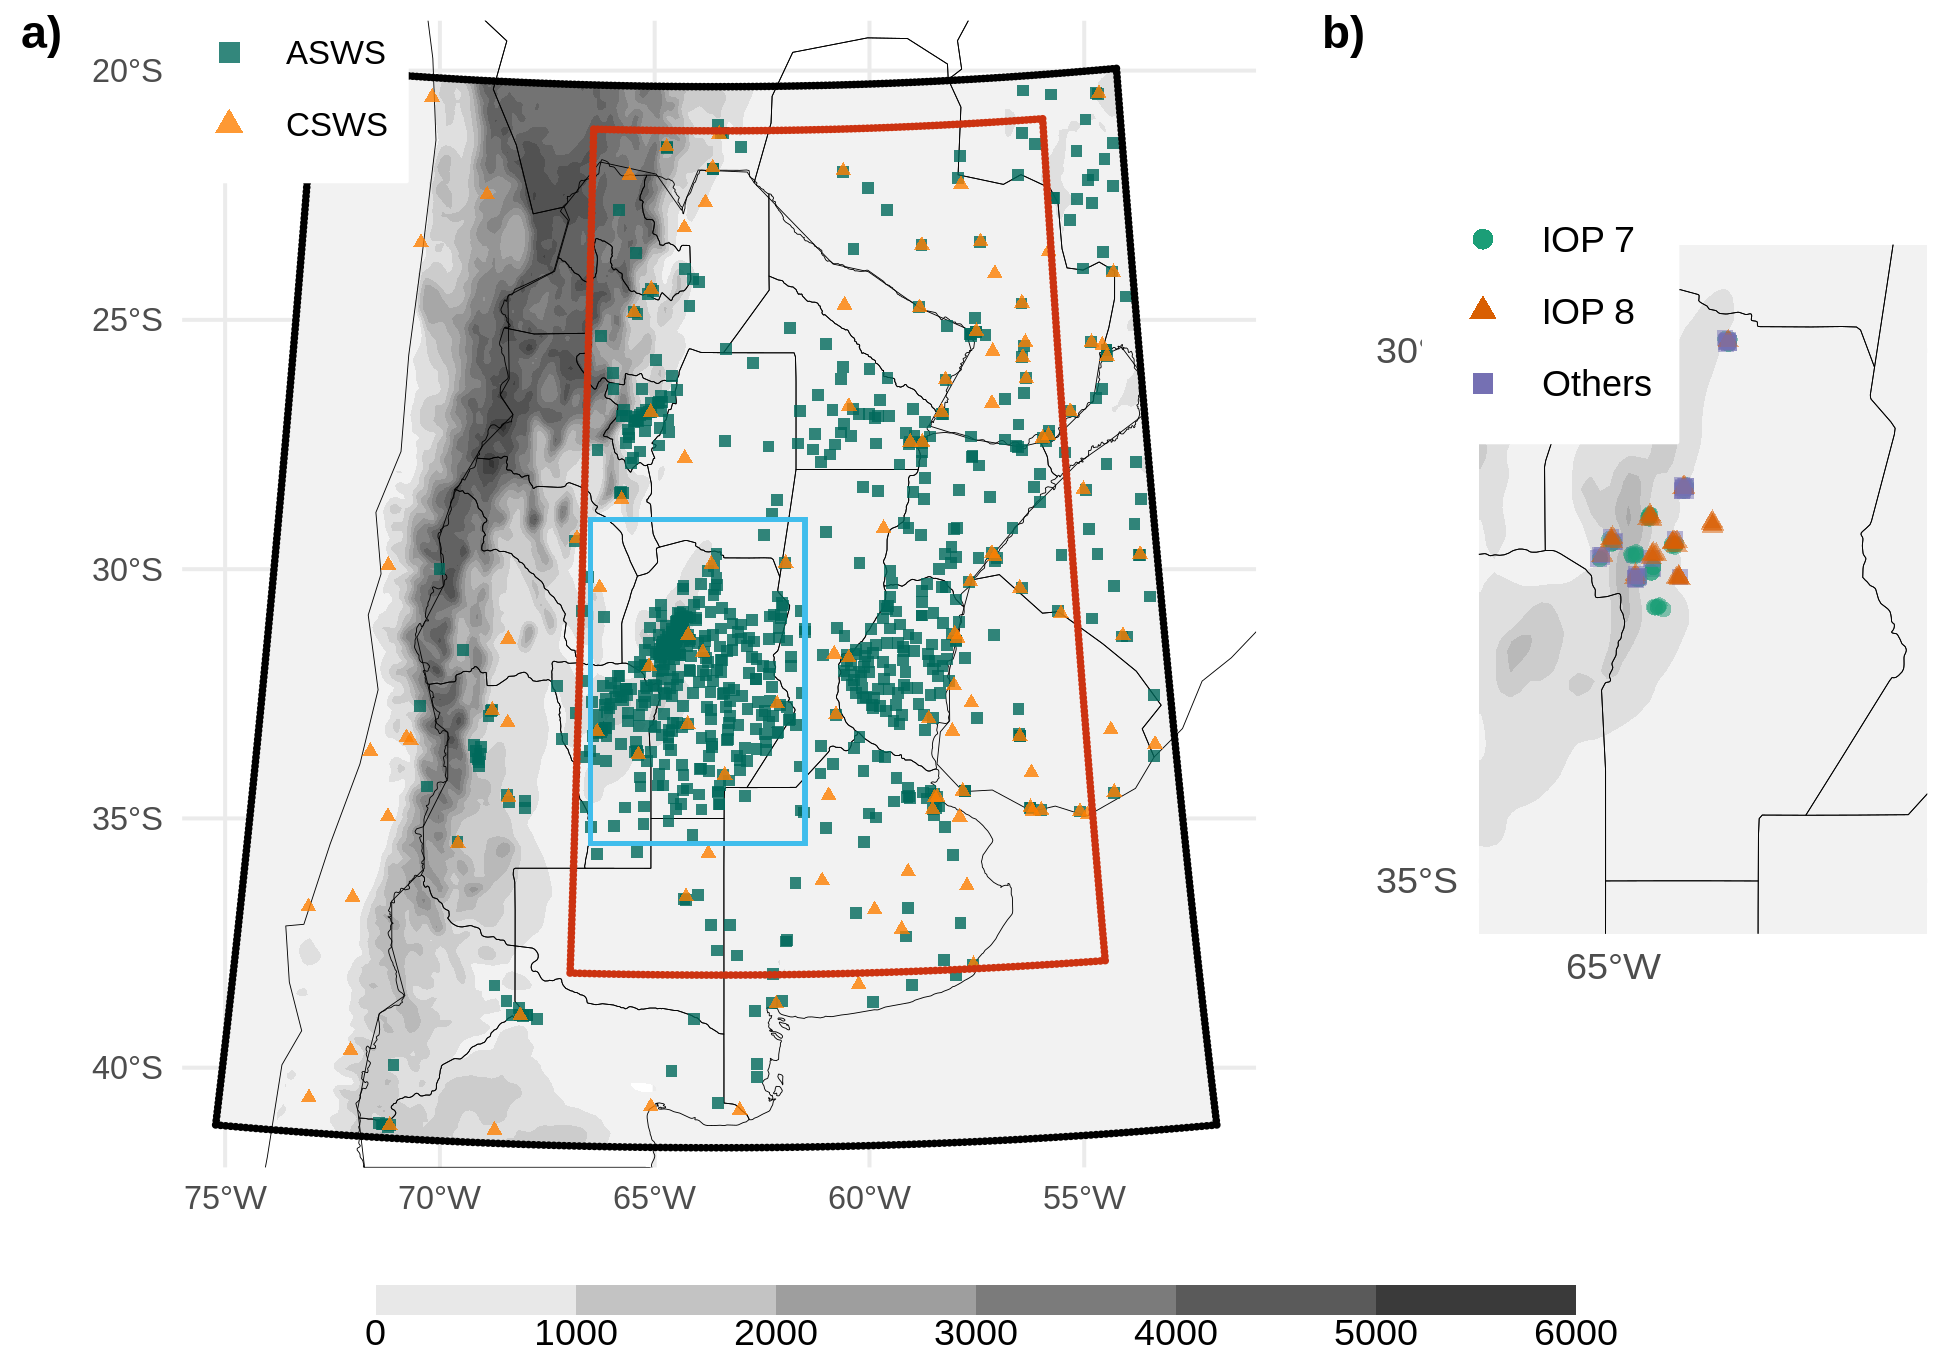
\includegraphics[width=1\linewidth]{../figures/dominio-1} \caption{a) The horizontal domain used on the simulations (black box), the inner domain used for the experiment comparison (red box), the region shown in b) (light blue box) and the locations of Automatic Surface Weather Stations (ASWS, green squares) and Conventional Surface Weather Stations (CSWS, orange triangles). b) Locations of radiosonde launches during the experiment, green dots corresponds to radiosondes launched during IOP 7, orange triangles are radiosondes launched during IOP 8 and purple square are radiosondes launched outside the IOP missions. The topography in meters is also shown (filled contours).}\label{fig:dominio}
\end{figure}

\hypertarget{observations}{%
\subsection{Observations}\label{observations}}

\hypertarget{conventional-and-satellite-derived-wind}{%
\subsubsection{Conventional and Satellite-derived wind}\label{conventional-and-satellite-derived-wind}}

The conventional and satellite-derived wind observations used are part of the Global Data Assimilation System (GDAS). We assimilated conventional observations included in the Binary Universal Form for Representation of Meteorological Data (PREPBUFR) files generated at NCEP that consist of surface observations from conventional surface weather stations (CSWS) and ships and upper-air observations from radiosondes and aircraft. The orange triangles in Figure \ref{fig:dominio}a, are the surface stations and ship locations included in this experiment. The orange triangles in Figure \ref{fig:dominio} a), are the surface station locations included in this experiment. The frequency of these observations varied between 1 hour for surface stations and 12/24 hours for most radiosondes in the region.

Satellite-derived wind observations also come from GDAS and include information from GOES-16 (estimated from the visible, infrared, and water vapor channels) and METEOSAT 8 and 11 (visible and water vapor channels). Due to the domain covered by each of these satellites, GOES-16 is the primary source of satellite-derived winds (99 \% of the observations).

We used additional conventional observations from 866 Automatic Surface Weather Stations (ASWS) that are part of various public and private automatic station networks over Southern South America and are included in the RELAMPAGO Data Set repository (Garcia et al., 2019). These stations are indicated as green squares in Figure \ref{fig:dominio}a. They have higher spatial coverage than the CSWS and a sampling frequency of 10 minutes in most cases. The variables measured by the stations varied between networks; all stations measure temperature, but only 395 stations provide humidity, 422 provide pressure and 605 provide wind information.

Table \ref{tab:table-obs} lists all the observation types (i.e., pressure, temperature, specific humidity, and wind) available for each source, together with their associated errors. The observation errors were specified following the GSI default configuration. In some cases, the error varies with height and it depends on the specific platform (aircraft and satellite-derived wind). In terms of quality control, a gross check was performed by the observation operator by comparing the innovation (the difference between the observation and the model-simulated observation based on the first-guess) with a predefined threshold (also included in Table \ref{tab:table-obs}).

\begin{table}

\caption{\label{tab:table-obs}Characteristics of the assimilated observations: The code for each observation type and it source, the available variables, the observation error and the gross check thresholds used.}
\centering
\fontsize{6}{8}\selectfont
\begin{tabular}[t]{>{\raggedright\arraybackslash}p{3.5em}>{\raggedright\arraybackslash}p{4.5em}>{\raggedright\arraybackslash}p{5em}>{\raggedright\arraybackslash}p{7em}>{\raggedright\arraybackslash}p{7em}}
\toprule
Code & Platform & Variable & Error & Gross check\\
\midrule
 &  & Pressure & 1-1.6 $hPa^*$ & 3.6 $hPa$\\

 &  & Temperature & 1.5 $K$ & 7 $K$\\

 &  & Specific humidity & 20 \% & 8 $gKg^{-1}$\\

\multirow{-4}{3.5em}{\raggedright\arraybackslash CSWS   ASWS} & \multirow{-4}{4.5em}{\raggedright\arraybackslash Surface weather stations} & Wind & 2.2 $ms^{-1}$ & 6 $ms^{-1}$\\
\cmidrule{1-5}
 &  & Pressure & 1.1-1.2 $hPa^{**}$ & 4 $hPa$\\

 &  & Temperature & 0.8-1.5 $K^*$ & 8 $K$\\

 &  & Specific humidity & 20 \% & 8 $gKg^{-1}$\\

\multirow{-4}{3.5em}{\raggedright\arraybackslash ADPUPA} & \multirow{-4}{4.5em}{\raggedright\arraybackslash Radiosondes} & Wind & 1.4-3 $ms^{-1}$* & 8 $ms^{-1}$\\
\cmidrule{1-5}
 &  & Temperature & 1.47-2.5 $K^+$ & 7 $K$\\

\multirow{-2}{3.5em}{\raggedright\arraybackslash AIRCFT} & \multirow{-2}{4.5em}{\raggedright\arraybackslash Aircrafts} & Wind & 2.4-3.6 $ms^{-1+}$ & 6.5-7.5 $ms^{-1+}$\\
\cmidrule{1-5}
ASCATW & Advance Scatterometers & Wind & 1.5 $ms^{-1}$ & 5 $ms^{-1}$\\
\cmidrule{1-5}
 &  & Pressure & 1.3 $hPa$ & 4 $hPa$\\

 &  & Temperature & 2.5 $K$ & 7 $K$\\

 &  & Specific humidity & 20 \% & 8 $gKg^{-1}$\\

\multirow{-4}{3.5em}{\raggedright\arraybackslash SFCSHP} & \multirow{-4}{4.5em}{\raggedright\arraybackslash Ships and Buoys} & Wind & 2.5 $ms^{-1}$ & 5 $ms^{-1}$\\
\cmidrule{1-5}
SATWND & Satellite-derived winds & Wind & 3.8-8 $ms^{-1*+}$ & 1.3-2.5 $ms^{-1+}$\\
\bottomrule
\multicolumn{5}{l}{\rule{0pt}{1em}\textsuperscript{*} Observation error varied with height.}\\
\multicolumn{5}{l}{\rule{0pt}{1em}\textsuperscript{**} Observations over 600 hPa are rejected.}\\
\multicolumn{5}{l}{\rule{0pt}{1em}\textsuperscript{+} Observation error depends on the report type.}\\
\end{tabular}
\end{table}

\hypertarget{sat}{%
\subsubsection{Satellite radiances}\label{sat}}

Satellite radiances available through the GDAS data stream, consisting of infrared and microwave observations are used in this study. This includes the Advanced Microwave Sounding Unit - A (AMSU-A), Advanced Technology Microwave Sounder (ATMS), Microwave Humidity Sounder (MHS), High-resolution Infrared Radiation Sounder (HIRS/4), and 2 multispectral sensors, Atmospheric Infrared Sounder (AIRS) and Infrared Atmospheric Sounding Interferometer (IASI) over several satellite platforms (see Table 2). Since the regional domain is located in the mid-latitudes and the satellite platforms of interest are on polar orbits, each sensor scans the area only twice a day with a spatial coverage depending on the satellite swath. For this reason, the number of satellite observations varied significantly among cycles. This is evident in Figure 3 a) which shows the number of radiance observations assimilated at each analysis cycle as a function of pressure. In particular, the multispectral sensors provided between 100 and 10.000 observations for every scan every 12 hours, contributing 82 \% of the total amount of assimilated radiances in our experiment. The vertical location of each radiance observation was estimated as the model level at which its weighting function was maximized as calculated by CRTM. The multispectral sensors have good vertical coverage and are able to sense from the lower troposphere and up to the lower stratosphere. The channels whose maximum weighting function is located in the stratosphere were rejected due to the low model top (50 hPa) used in the experiments.

The channels accepted for assimilation and their associated error were defined using the default GSI configuration. The data preprocessing, which is an essential step in the assimilation of radiances, was performed within the GSI system for each sensor specifically. Firstly a spatial data thinning is applied using a 60 km grid following (Jones et al., 2013; Lin et al., 2017; Singh et al., 2016), where the observations to be assimilated are chosen based on their distance to the model grid points, on the observation quality (based on available data quality information) and on the number of available channels (from the same pixel and sensor) that passed the quality control. Also, observations over the sea are preferred over those over land or snow (Hu et al., 2018).

The thinned observations were then bias corrected. The bias correction (BC) has an air-mass dependent and an angle-dependent component (Zhu et al., 2014) and it is calculated as a multi-linear function of N predictors \(p_i(x)\), with associated coefficients \(\beta_i\). Then, the bias corrected brightness temperature can be obtained as:

\[\mathit{BT_{bc}} =\mathit{ BT} + \sum_{i = 0}^{N} \beta_i p_i (x)\]

GSI has a constant offset bias correction term (\(p_0 = 1\)) and the following predictors are the cloud liquid water content (CLW), the temperature lapse rate at the pressure of maximum weight, the square of the temperature lapse rate at the pressure of maximum weight, and the emissivity sensitivity. Scan angle-dependent bias is modeled as a 4th-order polynomial (Zhu et al., 2014).

In the GSI system, the \(\beta_i\) coefficients are trained using a variational estimation method which solves for the \(\beta_i\) that provides the best fit between the simulation and the observations. The coefficients initialized from the 18 UTC Nov 11, 2018, GFS system coefficients were trained during one week of continuous assimilation using the same setup as in the experiments described in the next section. Moreover, the assimilation system was configured to use a constant background error variance of 0.01 to avoid large adjustments in the estimated coefficients at each cycle.

In our experiments, only clear-sky observations are used. For microwave radiances, observations potentially contaminated by clouds are detected using the scattering and Liquid Water Path (LWP) indexes (Weston et al., 2019; Zhu et al., 2016). For the infrared channels cloud contaminated observations are detected using the transmittance profile calculated within the CRTM algorithms. Additionally, the GSI quality control for infrared sensors looks for observations over water with a large zenithal angle (over 60°) to reject channels near the visible range that can be contaminated with reflection. It also performs an emissivity check for observations over land for both infrared and microwave radiances.

\begin{table}

\caption{\label{tab:table-rad}List of the available sensors over several platforms, the number of accepted channels for the assimilation and the percentage of assimilated observations calculated over all radiance observations and all cycles.}
\centering
\fontsize{7}{9}\selectfont
\begin{tabu} to \linewidth {>{\raggedright}X>{\raggedright}X>{\raggedleft}X>{\raggedright}X}
\toprule
Sensor & Plataform & \makecell[r]{Assimilated\\channels} & \makecell[l]{Percentage\\over total}\\
\midrule
AIRS & AQUA & 118 & 39.37 \%\\
\cmidrule{1-4}
 & AQUA & 7 & 1.13 \%\\
\cmidrule{2-4}
 & N19 & 13 & 1.55 \%\\
\cmidrule{2-4}
 & N15 & 13 & 3.93 \%\\
\cmidrule{2-4}
 & N18 & 13 & 3.17 \%\\
\cmidrule{2-4}
\multirow[t]{-5}{*}{\raggedright\arraybackslash AMSUA} & METOP-A & 13 & 1.3 \%\\
\cmidrule{1-4}
 & N20 & 21 & 1.16 \%\\
\cmidrule{2-4}
\multirow[t]{-2}{*}{\raggedright\arraybackslash ATMS} & NPP & 21 & 0.86 \%\\
\cmidrule{1-4}
 & N19 & 14 & 1.79 \%\\
\cmidrule{2-4}
\multirow[t]{-2}{*}{\raggedright\arraybackslash HIRS4} & METOP-A & 14 & 1.37 \%\\
\cmidrule{1-4}
 & METOP-A & 174 & 40.07 \%\\
\cmidrule{2-4}
\multirow[t]{-2}{*}{\raggedright\arraybackslash IASI} & METOP-B & 174 & 2.94 \%\\
\cmidrule{1-4}
 & N19 & 5 & 0.44 \%\\
\cmidrule{2-4}
 & METOP-A & 5 & 0.46 \%\\
\cmidrule{2-4}
\multirow[t]{-3}{*}{\raggedright\arraybackslash MHS} & METOP-B & 5 & 0.44 \%\\
\bottomrule
\end{tabu}
\end{table}



\begin{figure}
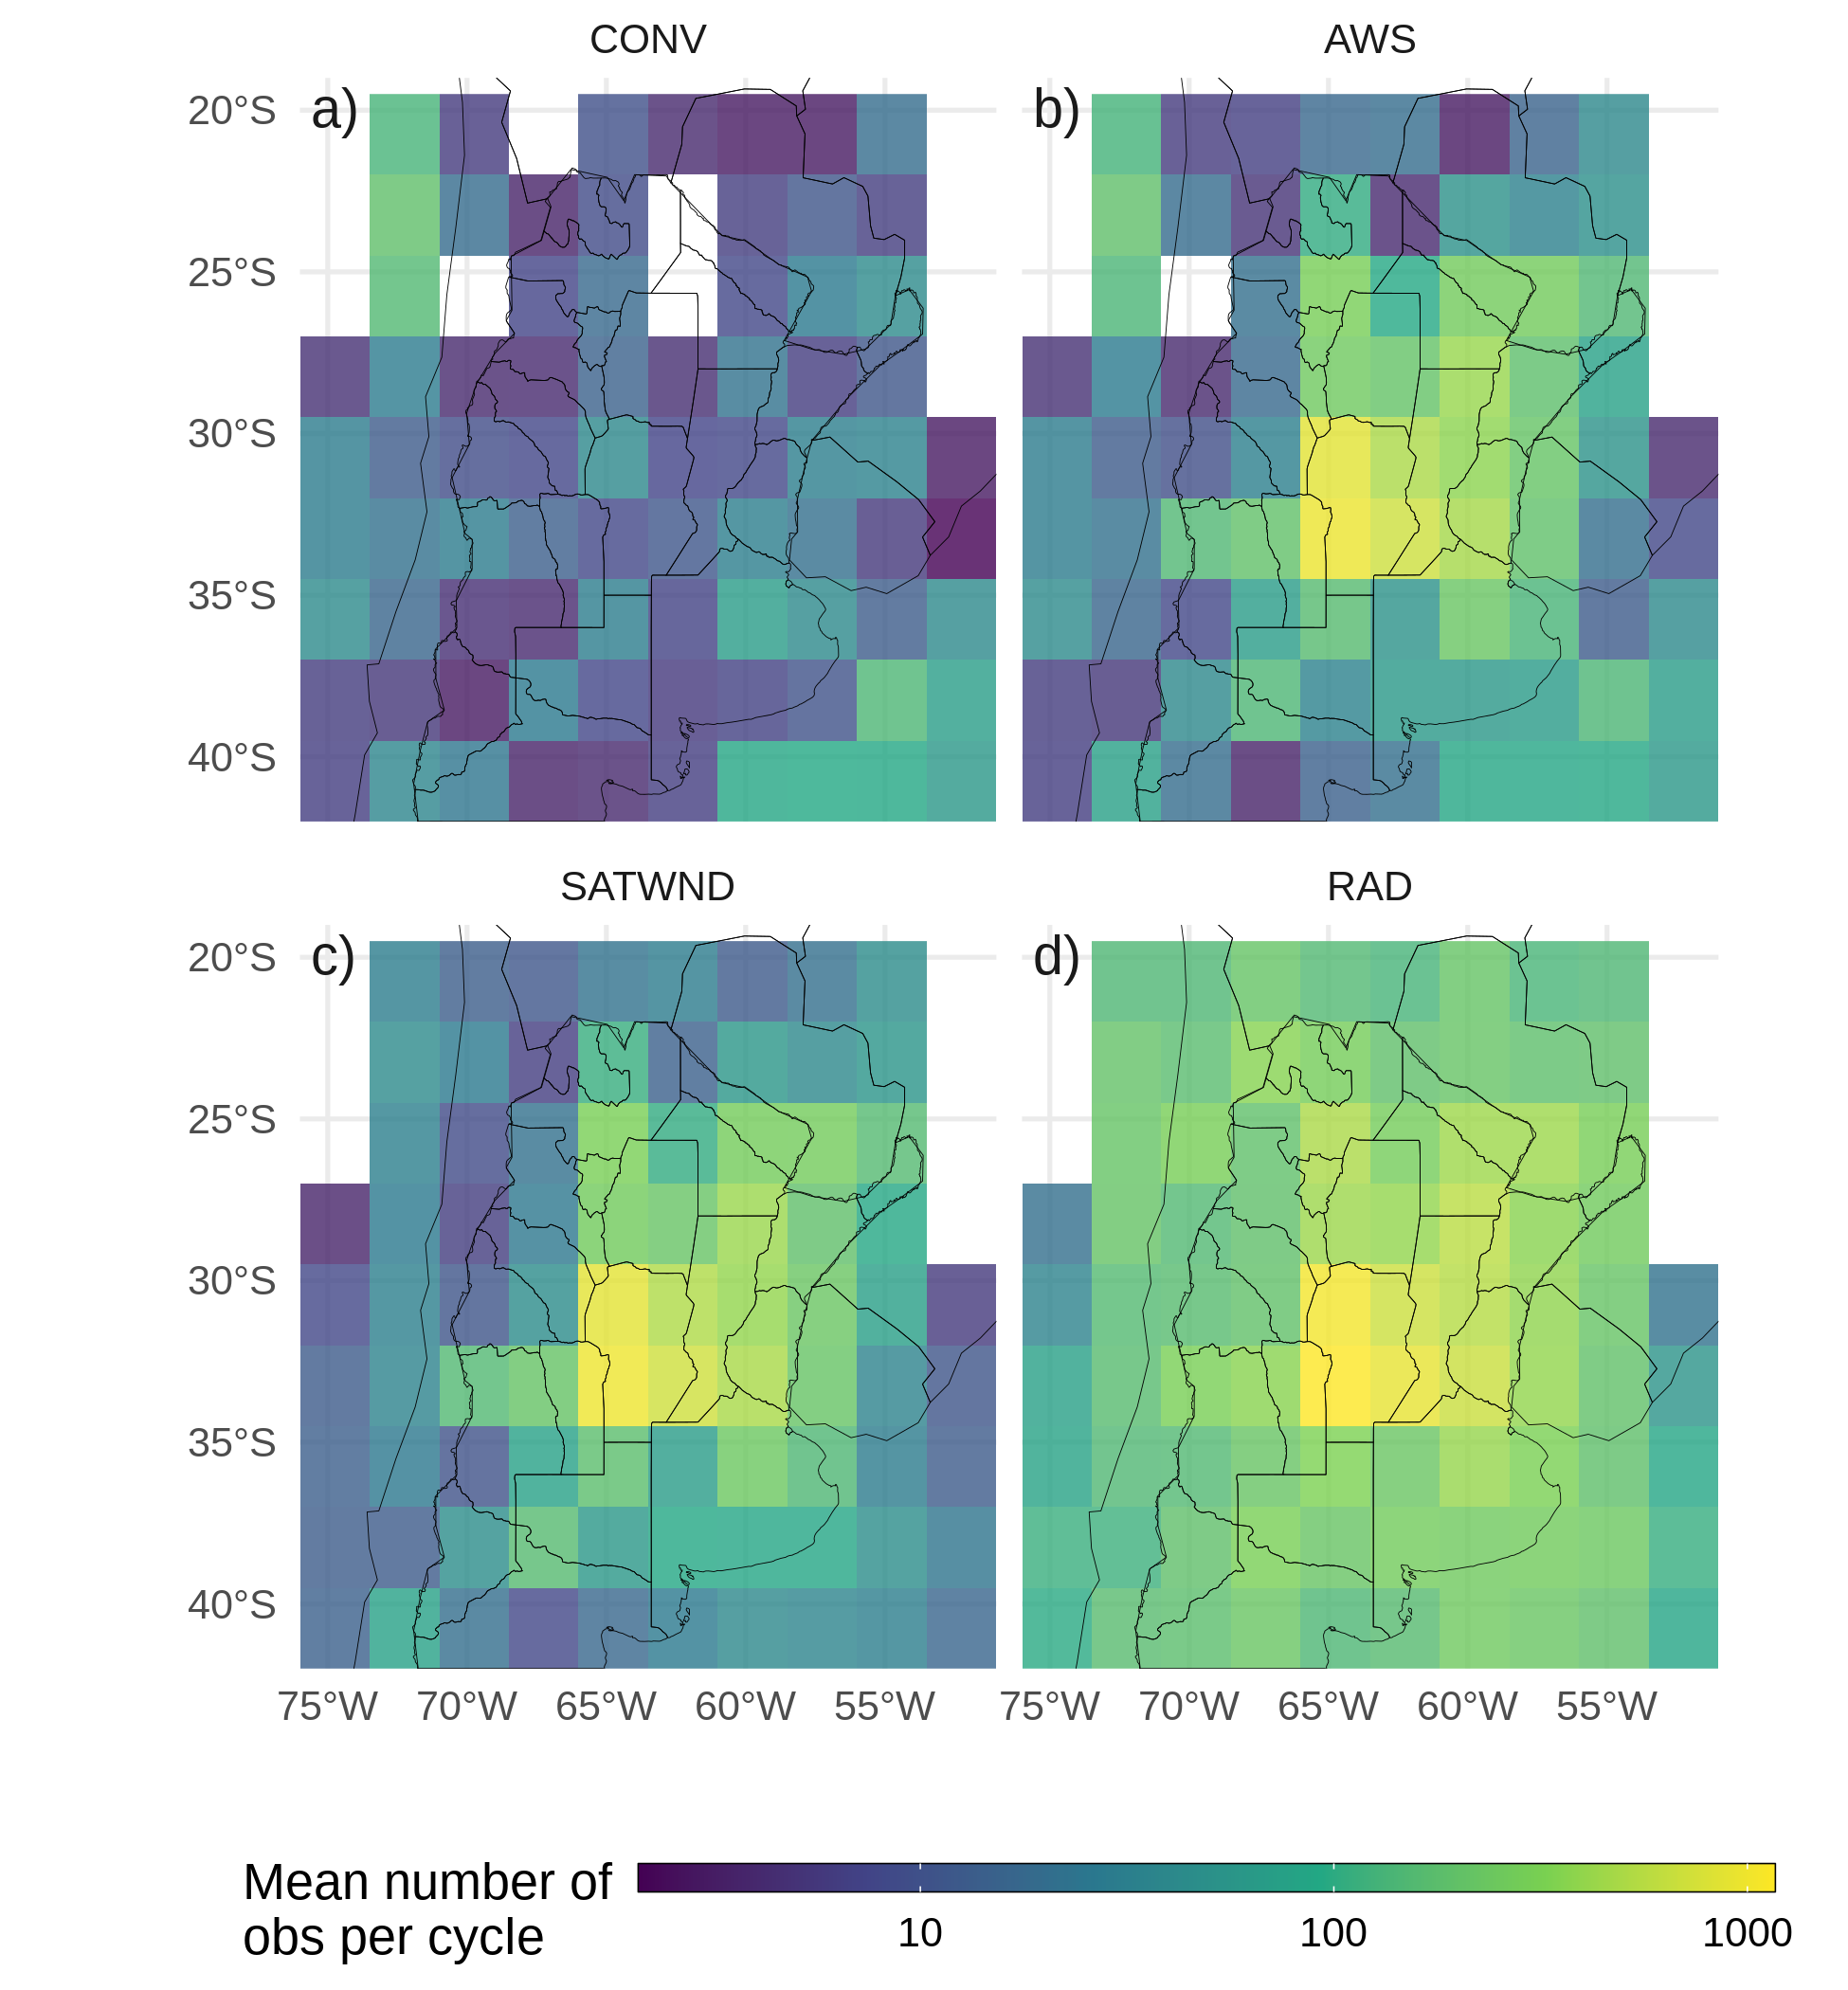
\includegraphics[width=1\linewidth]{../figures/obs-horizontal-1} \caption{Horizontal spatial distribution of the mean available observations per analysis cycle for the a) CONV, b) AUT c) SATWND and d) RAD experiments calculate over 2.5\(^{\circ}\) boxes.}\label{fig:obs-horizontal}
\end{figure}



\begin{figure*}
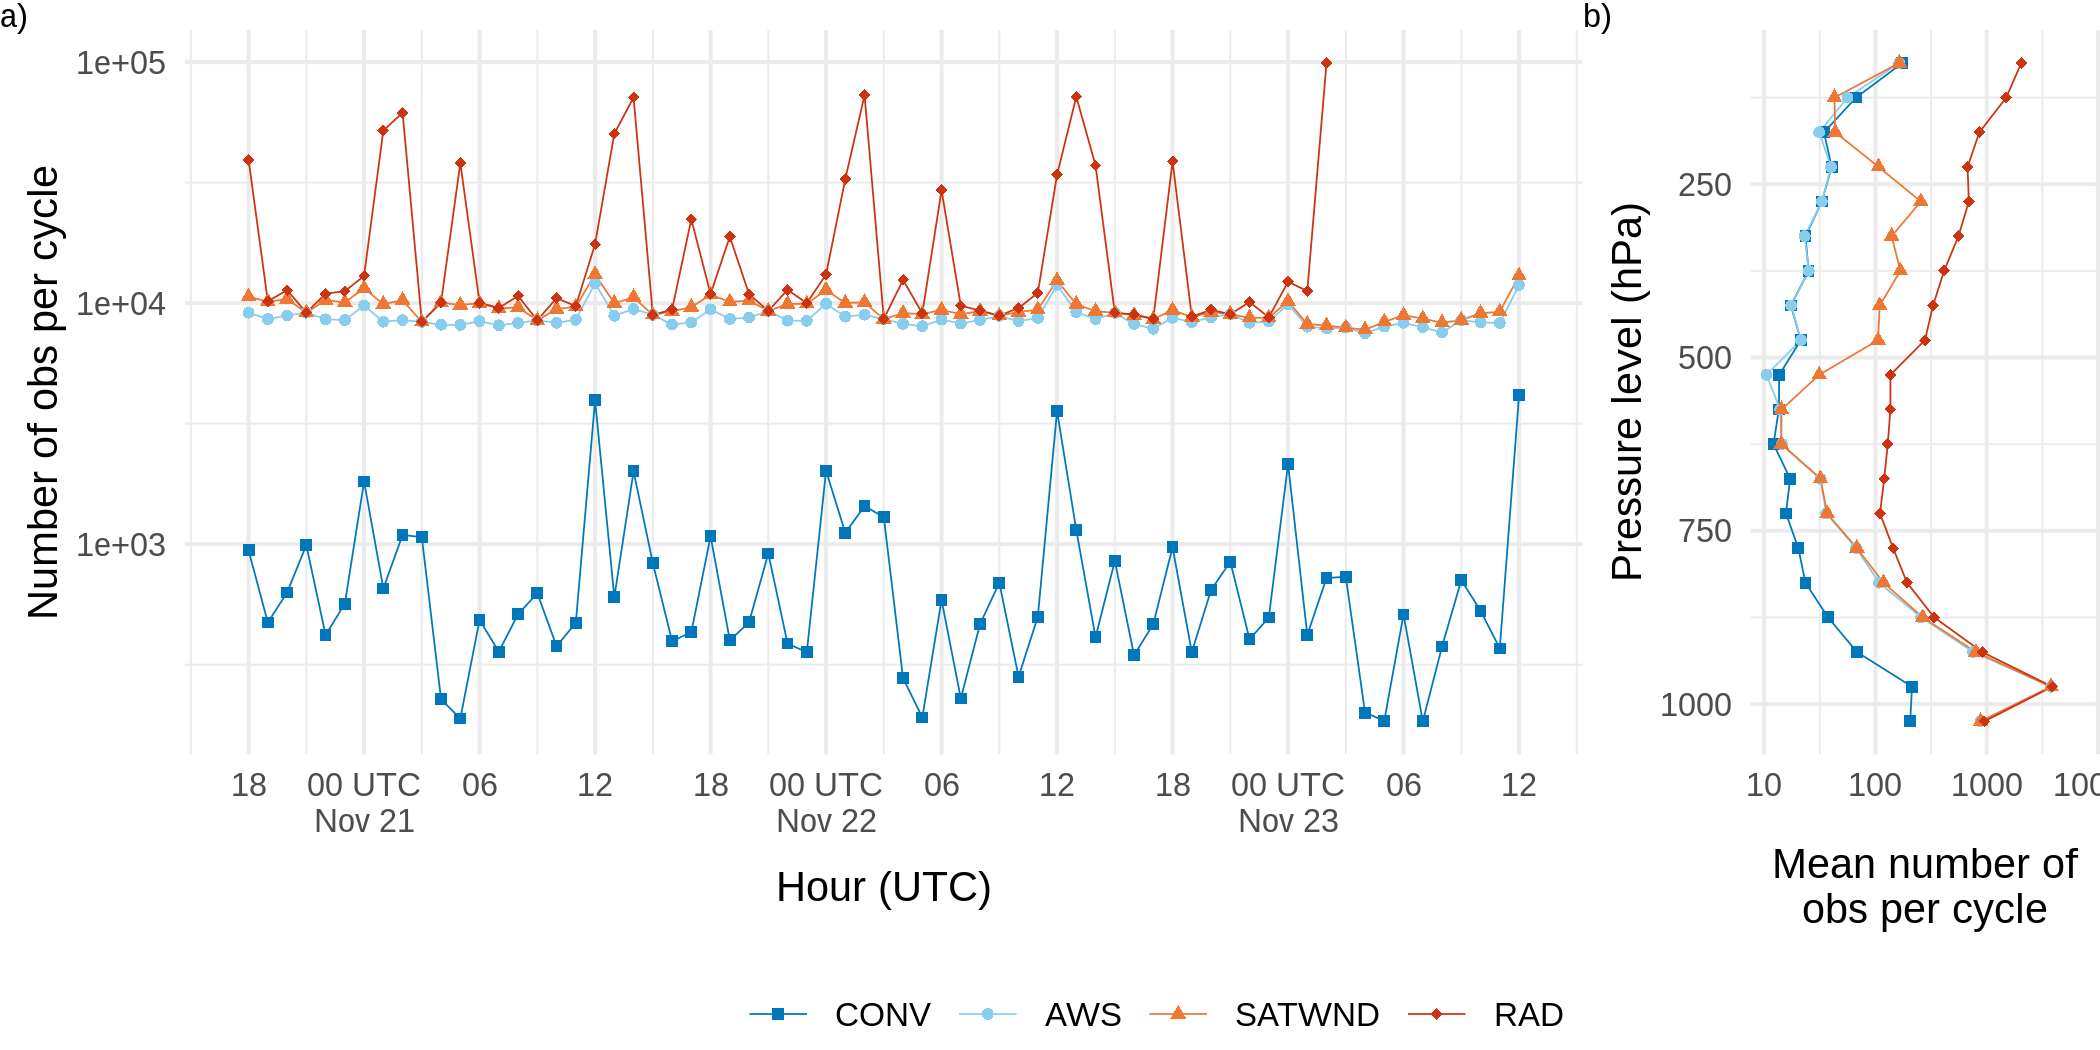
\includegraphics{../figures/obs-cycle-1} \caption{a) Number of assimilated observations per cycle and b) time averaged number of assimilated observations per cycle divided into 50 hPa-depth vertical layers for the CONV (blue squares and line), AUT (light blue dots and line), SATWND (orange triangles and line) and RAD (red diamond and line) experiments.}\label{fig:obs-cycle}
\end{figure*}

\hypertarget{validation-dataset}{%
\subsubsection{Validation dataset}\label{validation-dataset}}

To evaluate the performance of the ensemble-based data assimilation system presented in this article, we use the following observations datasets:

\begin{itemize}
\item
  The Multi-Network Composite Highest Resolution Radiosonde Data (Earth Observing Laboratory, 2020) from the RELAMPAGO field campaign database consisting of high-resolution radiosondes launched from several locations during the Intensive Observation Periods (IOP) along with the operational measurements. Only the soundings that did not enter the assimilation system were used for validation. The experiment period covers IOP missions 7 and 8 during which 74 radiosondes were launched in a small area near the center of the experimental domain (Figure \ref{fig:dominio}b).
\item
  The Satellite precipitation estimation IMERG Final Run with 0.01\(^{\circ}\) spatial resolution and 30 minutes temporal resolution (Huffman et al., 2018) was used as a reference state to validate the skill of 1-hour forecasts to represent the precipitation over the domain.
\item
  Radar observations are used to perform a qualitative and visual assessment of the convection features. The data comes from 9 radars located on the domain and is provided by the Argentine C-band Doppler dual-polarization weather radar network (de Elía et al., 2017) with a temporal frequency of 10 minutes. For this work, only the maximum reflectivity in the column (COLMAX) field closest to the analysis time was used.
\end{itemize}

\hypertarget{experimental-design}{%
\subsection{Experimental design}\label{experimental-design}}

To investigate the impact of different observations upon the analysis, four data assimilation experiments were performed using different observation sets (Table \ref{tab:table-exp}). The CONV experiment uses only convectional observations from PREPBUFR. In a second experiment, referred to as AUT, we assimilate all the observations included in CONV plus the 10-minute frequency surface observations from ASWS. In the third experiment, referred to as SATWND, we assimilate all the observations of the AUT experiment and the satellite-derived motion winds. Finally, a fourth experiment referred to as RAD assimilates all available clear-sky observations from sensors onboard polar orbit satellites as described in Section \ref{sat}.

The horizontal distribution of the average number of assimilated observations per cycle in each experiment is shown in Figure \ref{fig:obs-horizontal}. The larger number of assimilated observations over the center and east of the domain corresponds to the ASWS observations. In this region, we observed high values of precipitation during Nov 22 and is associated with the inflow of moisture by the South American low level jet. In Figure \ref{fig:obs-cycle}a the number of assimilated observations over time is shown. Local maxima at 12 and 00 UTC found mainly in CONV is produced by the operational soundings. The strong variability in the number of radiance observations per cycle is also noticeable and depends on the satellite coverage. The maxima after 12 and 00 UTC in RAD correspond to the contribution of the multispectral sensors. The vertical distribution of the mean number of observations per cycle (Figure \ref{fig:obs-cycle}b) shows a maximum in low levels due to the ASWS observations. Satellite-derived winds available in this particular case are maximum at the upper troposphere (between 500-250 hPa). Above 850 hPa, most of the observations correspond to radiance observations.

All the assimilation experiments start at 18 UTC Nov 20, 2018 and continue until 12 UTC Nov, 23 (totaling 67 hours/assimilation cycles). The initial ensemble is generated from a spin-up run without assimilating observations performed between 12 UTC and 18 UTC Nov, 20 (Figure \ref{fig:cycle}).

\begin{table}

\caption{\label{tab:table-exp}Observation types assimilated in each experiment.}
\centering
\begin{tabu} to \linewidth {>{\raggedright\arraybackslash}p{8em}>{\centering\arraybackslash}m{2.5em}>{\centering\arraybackslash}m{2.5em}>{\centering\arraybackslash}m{3em}>{\centering\arraybackslash}m{3em}}
\toprule
Obs type & CONV & AUT & SATWND & RAD\\
\midrule
Conventional (PREPBUFR) & x & x & x & x\\
Conventional (ASWS) &  & x & x & x\\
Satellite-derived winds &  &  & x & x\\
Radiances &  &  &  & x\\
\bottomrule
\end{tabu}
\end{table}



\begin{figure}
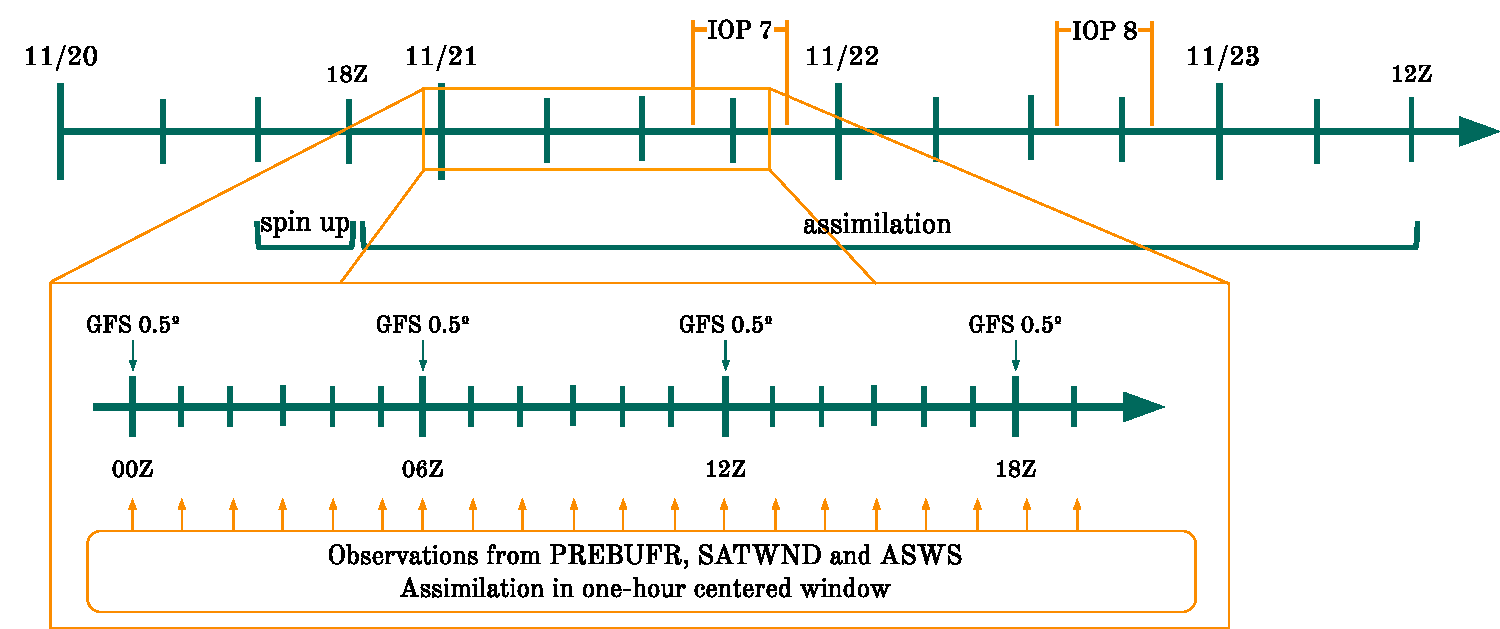
\includegraphics[width=1\linewidth]{/home/paola.corrales/mesoda/analysis/figures/analysis_cycle} \caption{Diagram of the analysis cycles between Nov 20th, 18 UTC and Nov 23 12 UTC plus and spin up period of 6 hours. The zoomed section shows the hourly assimilation hour that is performed within a one-hour centered window and new boundary conditions from GFS every 6 hours. The two Intensive Observation Periods (IOP) missions from the RELAMPAGO Field Campaign are shown.}\label{fig:cycle}
\end{figure}

\hypertarget{verification-methods}{%
\subsection{Verification methods}\label{verification-methods}}

A set of metrics are selected to evaluate different aspects of the analysis obtained in the experiments conducted in this paper. These aspects include a validation of how the uncertainty is quantified in the first-guess and in the analysis and how different experiments fit an independent set of observations that are not assimilated.

To evaluate the consistency of the uncertainty quantification in the first-guess and in the analysis we use the Reduced Centered Random Variable (RCRV, Candille et al. (2007)) which is defined as:

\[RCRV = \frac{x_o - m}{\sqrt{\sigma_o^2 + \sigma^2}}\]

where \(x_o\) is the observation and its error \(\sigma_o\), the mean \(m\), and the standard deviation \(\sigma\) of the ensemble.
The average of \(RCRV\) computed over all the realizations represents the bias of the ensemble mean with respect to the observations normalized by the estimated uncertainty:

\[\mathit{mean RCRV} = E[RCRV]\]

The standard deviation of the \(RCRV\) or \(sd RCRV\) measures the agreement of the ensemble spread and the observational error with respect to the distance between the ensemble mean and the observations, and then the systematic over- or under- dispersion of the ensemble:

\[\mathit{sd RCRV} = \sqrt{\frac{M}{M -1}E[(\mathit{RCRV} - \mathit{mean RCRV})^2]}\]

where \(M\) is the sample size. A reliable system will have no bias (\(mean RCRV = 0\)), and a standard deviation equal to 1 (\(sd RCRV = 1\)). If the ensemble has a positive (negative) bias, \(mean RCRV\) will be positive (negative). A \(sd RCRV > 1\) (\(sd RCRV < 1\)), indicates that the ensemble is underdispersive (overdispersive).

The fit of the first-guess and analysis to a set of independent observations is computed based on the Root Mean Square Error (RMSE) and the BIAS:

\[\mathit{RMSE} = \sqrt{\frac{1}{N}\sum_{i = 1}^{N} (X_i - O_i)^{2}}\]

\[\mathit{BIAS} = \frac{1}{N}\sum_{i = 1}^{N} (X_i - O_i)\]

where \(O\) and \(X\) stand for independent observations and the analysis respectively.

For the comparison of the first-guess' precipitation with the precipitation estimates, we compute a probabilistic Fraction Skill Score (FSS) for different sized sampling areas and thresholds, following Maldonado et al. (2021) and adaptations from Roberts (2008).

\[\mathit{FSS} = 1-\frac{\frac{1}{N}\sum_{i=1}^{N} ({P_x}_i-{P_o}_i)^{2}}{\frac{1}{N}\sum_{i=1}^{N} ({P_x}_i)^{2}+\frac{1}{N}\sum_{i=1}^{N} ({P_o}_i)^{2}} \]

where \({P_x}\) is the probability of occurrence of accumulated rainfall over a specified threshold computed from the ensemble and \({P_o}\) is 1 when the observed accumulated precipitation is over the same threshold and 0 otherwise. This probabilistic formulation uses the information from the full ensemble thus avoiding the smoothing effect of the ensemble mean which can particularly affect localized extreme precipitation values. The FSS was applied to the accumulated precipitation over 6 hr periods by adding the 1-hr accumulated precipitation forecasts over 6 consecutive assimilation cycles.

\hypertarget{computation-procedures}{%
\subsection{Computation procedures}\label{computation-procedures}}

We performed all analysis in this paper using the R programming language (R Core Team, 2020), using data.table (Dowle and Srinivasan, 2020) and metR (Campitelli, 2020) packages.
All graphics are made using ggplot2 (Wickham, 2009) and the paper was rendered using knitr and rmarkdown (Allaire et al., 2020; Xie, 2015). All the experiments were performed at the National Center for Atmospheric Research (NCAR) supercomputer Cheyenne (Computational and Information Systems Laboratory, 2019).

\hypertarget{results}{%
\section{Results}\label{results}}

\hypertarget{ensemble-reliability}{%
\subsection{Ensemble reliability}\label{ensemble-reliability}}

To investigate the ability of the first-guess ensemble mean to fit the observations taking into account the uncertainties of the forecast and the observations, we calculated the \(mean RCRV\) and the \(sd RCRV\) for the RAD experiment. As this experiment assimilates all types of observations used in this work, it is possible to analyze the reliability of the ensemble by comparing it with each type of observation. Figure 5 shows the \(sd RCRV\) for surface observations box-averaged to a 2.5° grid. The \(sd RCRV\) for wind observations (Figure \ref{fig:rcrv-sfc}a) is close to 1 suggesting a good agreement between the ensemble spread, the forecast error, and the observation error. For the temperature (Figure \ref{fig:rcrv-sfc}b), the results are similar except that for some areas to the west of the domain where the \(sd RCRV\) can be as high as 4.5. In this region, the mean innovation was overly large due to the complex terrain leading to large differences between the model topography and the station height.

Figure \ref{fig:rcrv-profile} shows the mean and standard deviation of the RCRV for the upper-air observations. Figure \ref{fig:rcrv-profile}a-b show the RCRV statistics for soundings (ADPUPA) and aircraft (AIRCAR and AIRCFT). Both ADPUPA and AIRCFR show a generally good agreement between the ensemble spread and the observation error. As sounding observations and their associated errors are known to be reliable, this result indicates that the ensemble has an appropriate spread. AIRCAR presents an irregular profile with \(sd RCRV\) values that suggest that the error for this type of observation is overestimated. ADPUPA and AIRCAR present a \(mean RCRV\) profile near zero on middle and upper levels but ADPUPA observations show a cold bias with respect to the model at low levels, a characteristic already studied in Ruiz et al. (2010) and Dillon et al. (n.d.).

For satellite-derived winds (Figure \ref{fig:rcrv-profile}c) in low levels, where there are not many observations available, the profiles of \(mean RCRV\) and \(sd RCRV\) shows a larger departure from the expected behavior with a negative bias and an overestimation of the observation error. Wind estimations derived from water vapor channels are abundant over 500 hPa where their bias is close to zero. The only exception are the EUMETSAT observations which contribute very little in the region.

The mean RCRV profiles calculated from the radiance observations (Figure \ref{fig:rcrv-profile}d) show almost no bias and the same happens if the \(mean RCRV\) is calculated over each channel of each sensor. This indicates that the bias correction algorithm works as expected. The \(sd RCRV\) values are less than 1 for all sensors possibly due to an overestimation of the observation errors to reduce the influence of potentially erroneous observations.

Overall these results indicate that the ensemble spread is consistent with the short-range forecast error and that systematic errors are relatively small for most of the observation types used in this work. Moreover, these results suggest the inflation parameter \(\beta = 0.9\) is adequate for the system.



\begin{figure}
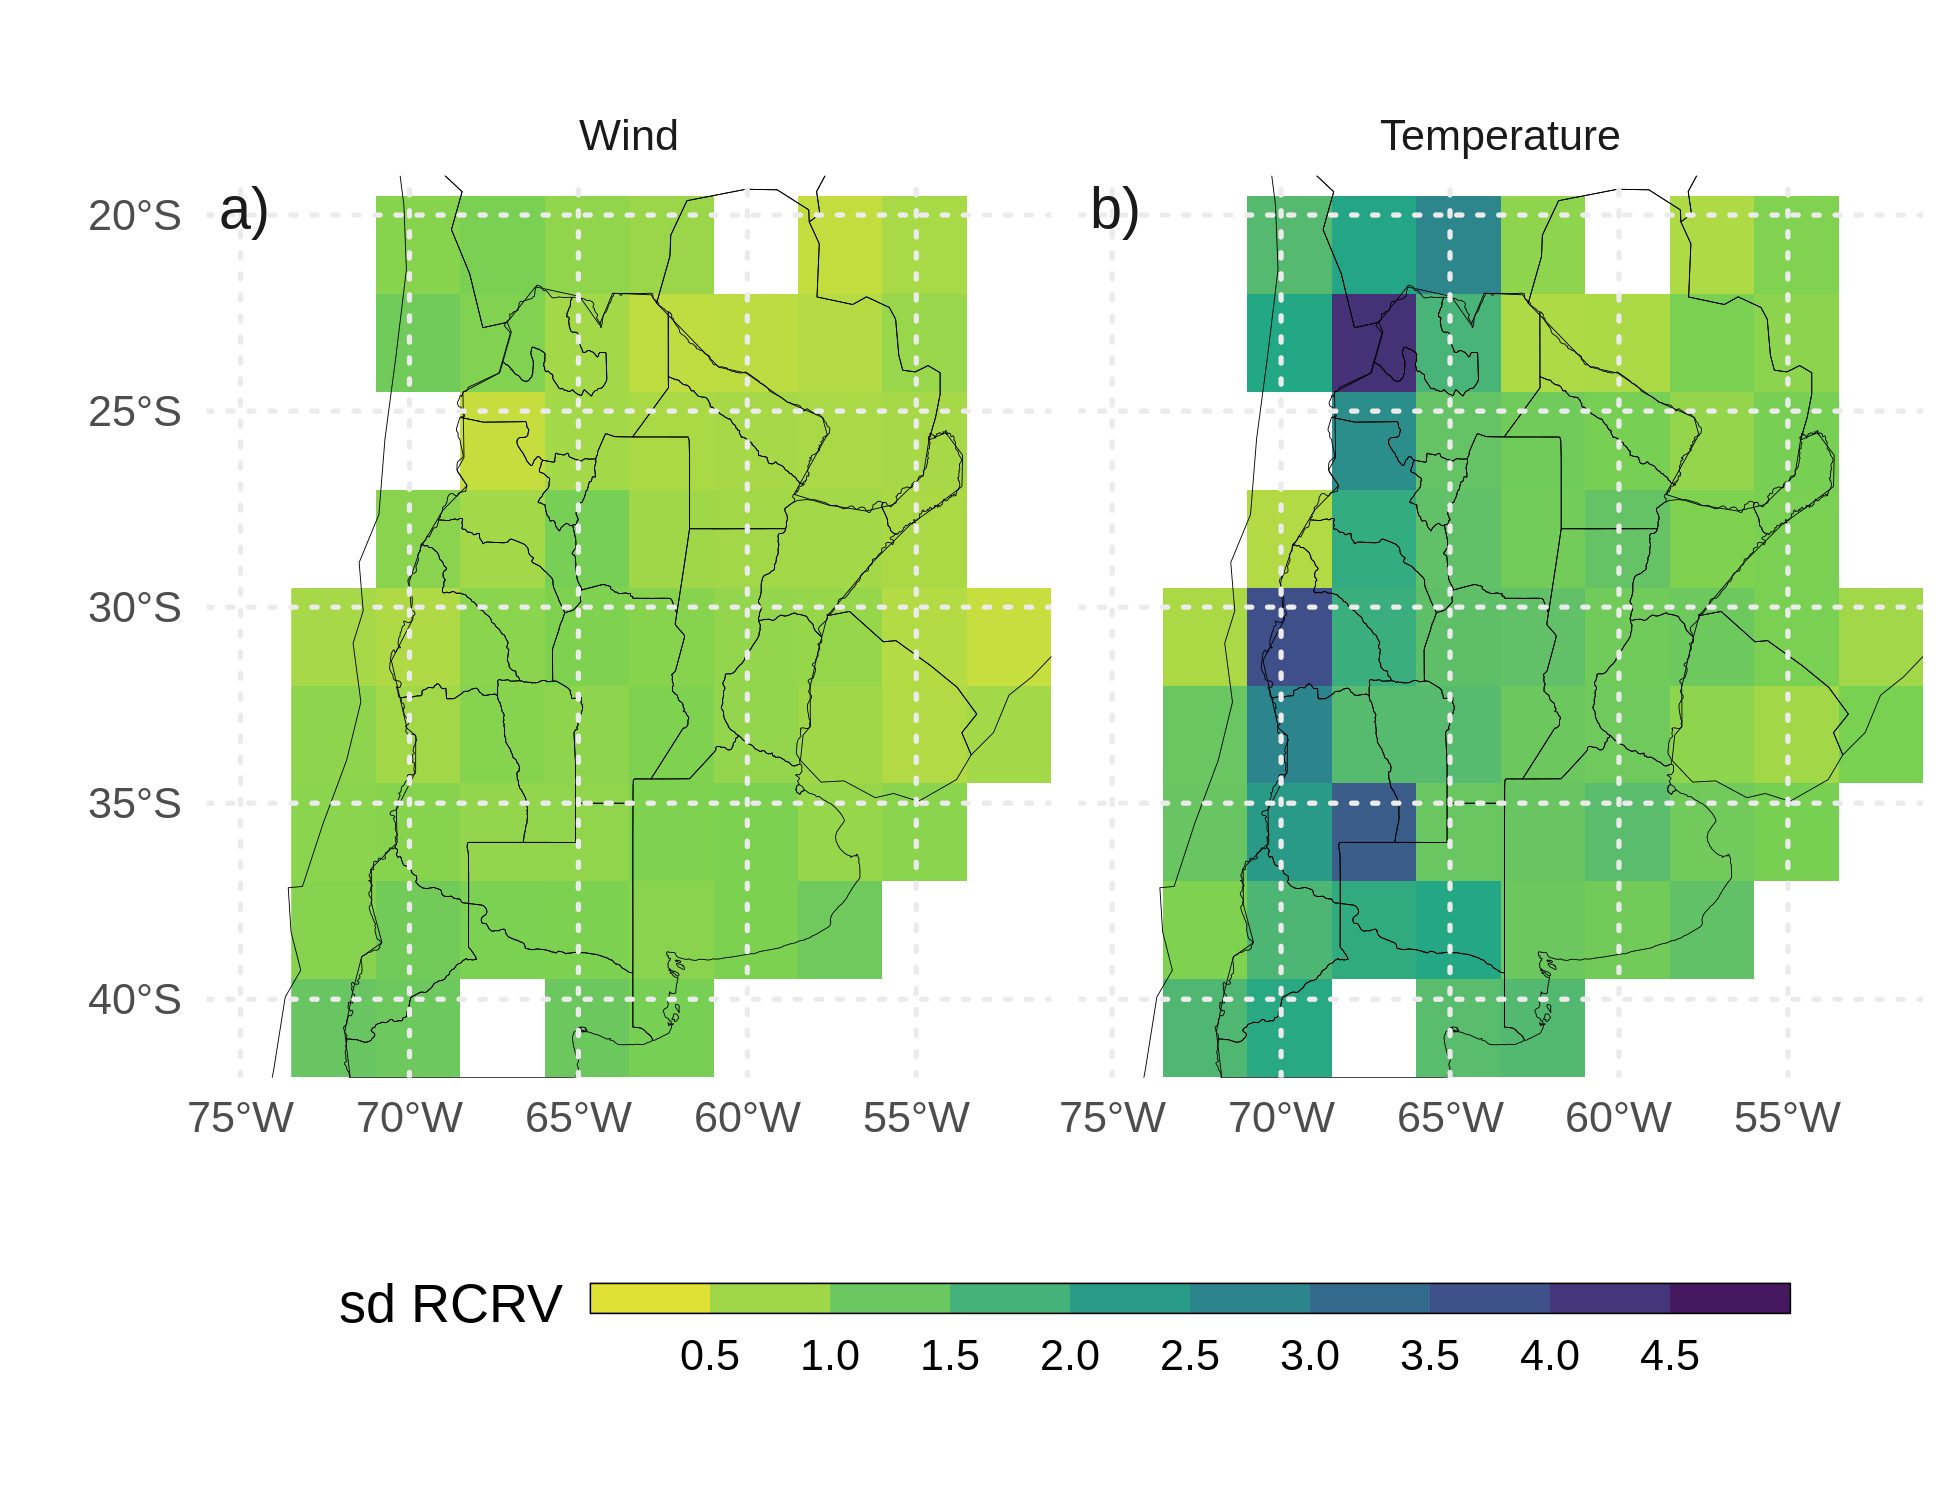
\includegraphics[width=1\linewidth]{../figures/rcrv-sfc-1} \caption{\(sd RCRV\) calculated for surface observations (from PREPBUFR and ASWS) of a) wind, and b) temperature, averaged over 2.5º boxes.}\label{fig:rcrv-sfc}
\end{figure}



\begin{figure*}
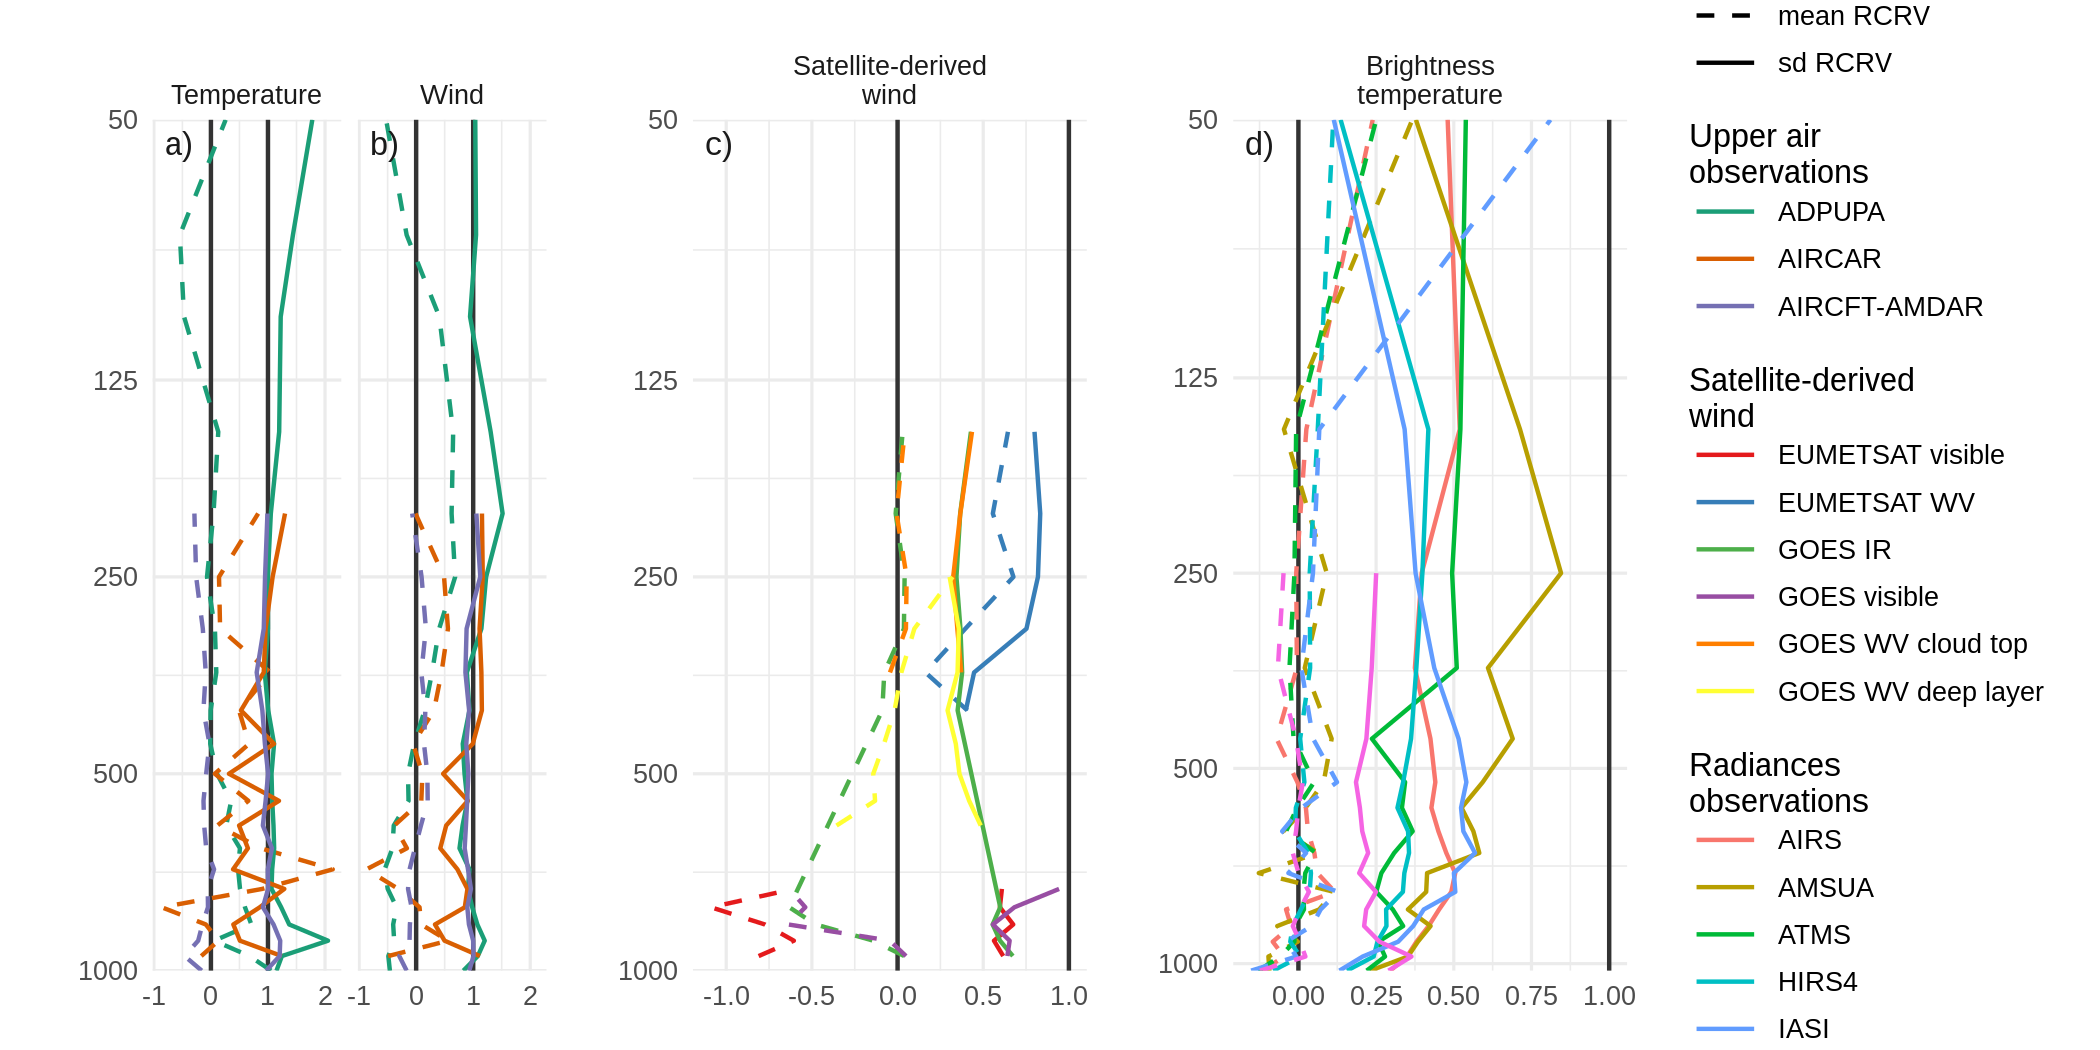
\includegraphics{../figures/rcrv-profile-1} \caption{Vertical profiles of \(mean RCRV\) (dash line) and \(sd RCRV\) (solid line) for a) temperature and b) wind of sounding and aircraft observations, c) satellite-derived wind observations, and d) brightness temperature observations.}\label{fig:rcrv-profile}
\end{figure*}

\hypertarget{impacts-of-assimilated-observations}{%
\subsection{Impacts of assimilated observations}\label{impacts-of-assimilated-observations}}

In this section, we present the impact of assimilating different observation types on variables which are particularly relevant for the occurrence of deep moist convection. The analysis is performed over a smaller domain (red box in Figure \ref{fig:dominio}a) to focus on the region most directly affected by the MCS. Figure \ref{fig:TQ-diff}a-c shows the difference between experiments in the spatially averaged vertical profile of temperature. By averaging the differences between two experiments we can isolate the systematic impact produced by different observing systems on the analyzed state. During the first day, the assimilation of ASWS observations results in a colder PBL. This cooling effect has a clear diurnal cycle being stronger during nighttime (Figure \ref{fig:TQ-diff}a). During the second day of the experiment, the impact of ASWS observations extends into the middle and upper troposphere coinciding with the mature stage of the MCS. The warm difference shown in AUT with respect to CONV in mid and upper levels is produced by the development of stronger convection in this experiment compared to CONV. This is a good example of how low-level information provided by surface weather stations can rapidly spread into the troposphere in the presence of deep moist convection. Figure \ref{fig:TQ-diff}b, indicates that SATWND observations have an almost negligible impact on the mean temperature through the experiment. This result is unexpected since mid-to-upper level winds can have a profound impact on the organization and evolution of MCSs over the region.
During the first day of the experiment, the assimilation of radiances produces a warming effect in the PBL which partially compensates for the cooling effect of ASWS observations. No clear systematic impact is found above the PBL during this period. During the second day, the impact of radiance observations is found through the troposphere with a distribution that is similar to the impact found in the AUT experiment but with the opposite sign.

Comparing the specific humidity in the experiments (Figure \ref{fig:TQ-diff}d-f) the impact of assimilating ASWS with larger spatial and temporal resolution is most significant at low levels (Figure \ref{fig:TQ-diff}d). The PBL in the AUT experiment is consistently moister than in the CONV experiment and this is enhanced during the nighttime. The increase in low-level moisture by a denser surface network is consistent with previously reported dry biases in the WRF model over the region (Ruiz et al., 2010). We found that the moistening of the PBL is mainly driven by the covariance between temperature and specific humidity within the PBL. In our experiment and over the center of the domain, this covariance remains negative, increasing low-level moisture as the observations introduce negative temperature corrections. As for the temperature, the systematic impact of satellite-derived winds is small and only important after 18 UTC Nov, 21 at low levels. Figure \ref{fig:TQ-diff}f shows that radiances reduce low-middle level moisture during the first day of the experiment. The drying effect extends to lower-middle levels during the second day of the experiment coinciding with the development of the MCS between 00 and 12 UTC Nov, 22.

The impacts on the wind components are shown in Figure Figure \ref{fig:UV-diff} along with the corresponding averaged wind component in the experiment with the largest number of assimilated observations. The assimilation of ASWS produces an increase of zonal wind and a decrease of meridional wind at low levels during the first two days of analysis. There is a diurnal cycle in the impact of surface weather stations on the meridional velocity (Figure \ref{fig:UV-diff}d) with a stronger reduction of the northerly wind during night hours. This indicates that surface observations are reducing the intensity of the low level jet present in the pre-convective environment. After 18 UTC Nov, 22 the opposite effect is observed when the MCS is moving through the domain. After the initiation of the convective cells, the systematic impact on the wind field is larger at mid and upper levels. During Nov 22 and 23 the impact of assimilating ASWS produces an increase of northerly wind in upper levels. This could be a consequence of a stronger MCS with an increased polar side upper level outflow. Satellite-derived wind observations produce the largest impact in mid-to-upper levels where the number of observations is larger, however, the systematic impact is overall smaller than the one produced by assimilating data from ASWS.

The assimilation of radiances produced a reduction in the westerly wind compared with respect to SATWIND in low and upper levels (Figure \ref{fig:UV-diff}c and f). For the meridional wind, these observations produce an enhancement on average of the northerly low-level flow of \(1 ms^{-1}\), opposite to what is generated by the assimilation of ASWS observations. On upper levels and during Nov 22 and 23 the average impact of assimilating radiances is a decrease in the wind. When we look at the meridional wind field at 200 hPa at different times, we observed that the outflow from the MCS is even more intense than in the other experiments while the southerly wind ahead of the MCS also increases producing in average a reduction of the northerly wind present in Figure \ref{fig:UV-diff}f.~

To investigate how changes in the PBL can modify the pre-convective environment we compare the horizontal distribution of the low level northerly flow, precipitable water, low level temperature, and CAPE for the analysis at 00 UTC Nov, 22 (after 30 assimilation cycles). At that moment the first convective cells were developing on the southern region of the domain along the cold front. Figure \ref{fig:summary-fields}a shows the precipitable water (shaded) and the vertically averaged low-level meridional wind component (contours). We found that the moist tongue extending over the northern part of the domain is enhanced by the assimilation of denser surface observations. The moisture increase is particularly stronger at the southern tip of this tongue, just ahead of the cold front where convection initiation was taking place. AUT and SATWND experiments are very similar, with values of precipitable water over 55 \(kgm^{-2}\) north of 30\(^{\circ}\)S and a similar vertical distribution of specific humidity (not shown). RAD has lower precipitable water content than AUT and SATWND but higher than CONV. The distribution of moisture at low levels in RAD seems to be the result of the combination of the moistening effect of assimilating ASWS -- partially compensated by the assimilation of radiance observations -- and a reduced meridional moisture transport due to the weaker northerly flow over the center of the domain compare to CONV.

The potential temperature on the PBL (Figure \ref{fig:summary-fields}b) resembles the characteristics observed on the temperature profiles in Figure \ref{fig:TQ-diff}a-c.~On average the PBL in AUT and SATWND is colder than in CONV while RAD shows a warmer PBL than AUT due to the assimilation of radiance observations. Figure \ref{fig:summary-fields}c shows the most unstable convective available potential energy (MCAPE, shaded) and the 0 to 6 \(km\) wind shear. The values of MCAPE in CONV do not exceed 2000 \(JKg^{-1}\) while the rest of the experiments show maximum MCAPE over 4000 \(JKg^{-1}\). MCAPE in the RAD experiment is lower compared to AUT or SATWND. This is consistent with less humidity in the PBL with respect to these experiments and may be partially compensated by a slightly warmer PBL in the RAD experiment. The 0-6 km wind shear is more intense in AUT, SATWND, and RAD reaching values over 15 \(ms^{-1}\) at the southern tip of the region with positive MCAPE values. Moreover, in this same region, these experiments show larger MCAPE values. Wind shear over 15 \(ms^{-1}\) have been associated with the development of more intense and organized MCSs (Chen et al., 2015) and also with conditions favorable for supercells (Markowsky and Richardson, 2010).



\begin{figure*}[t]

{\centering 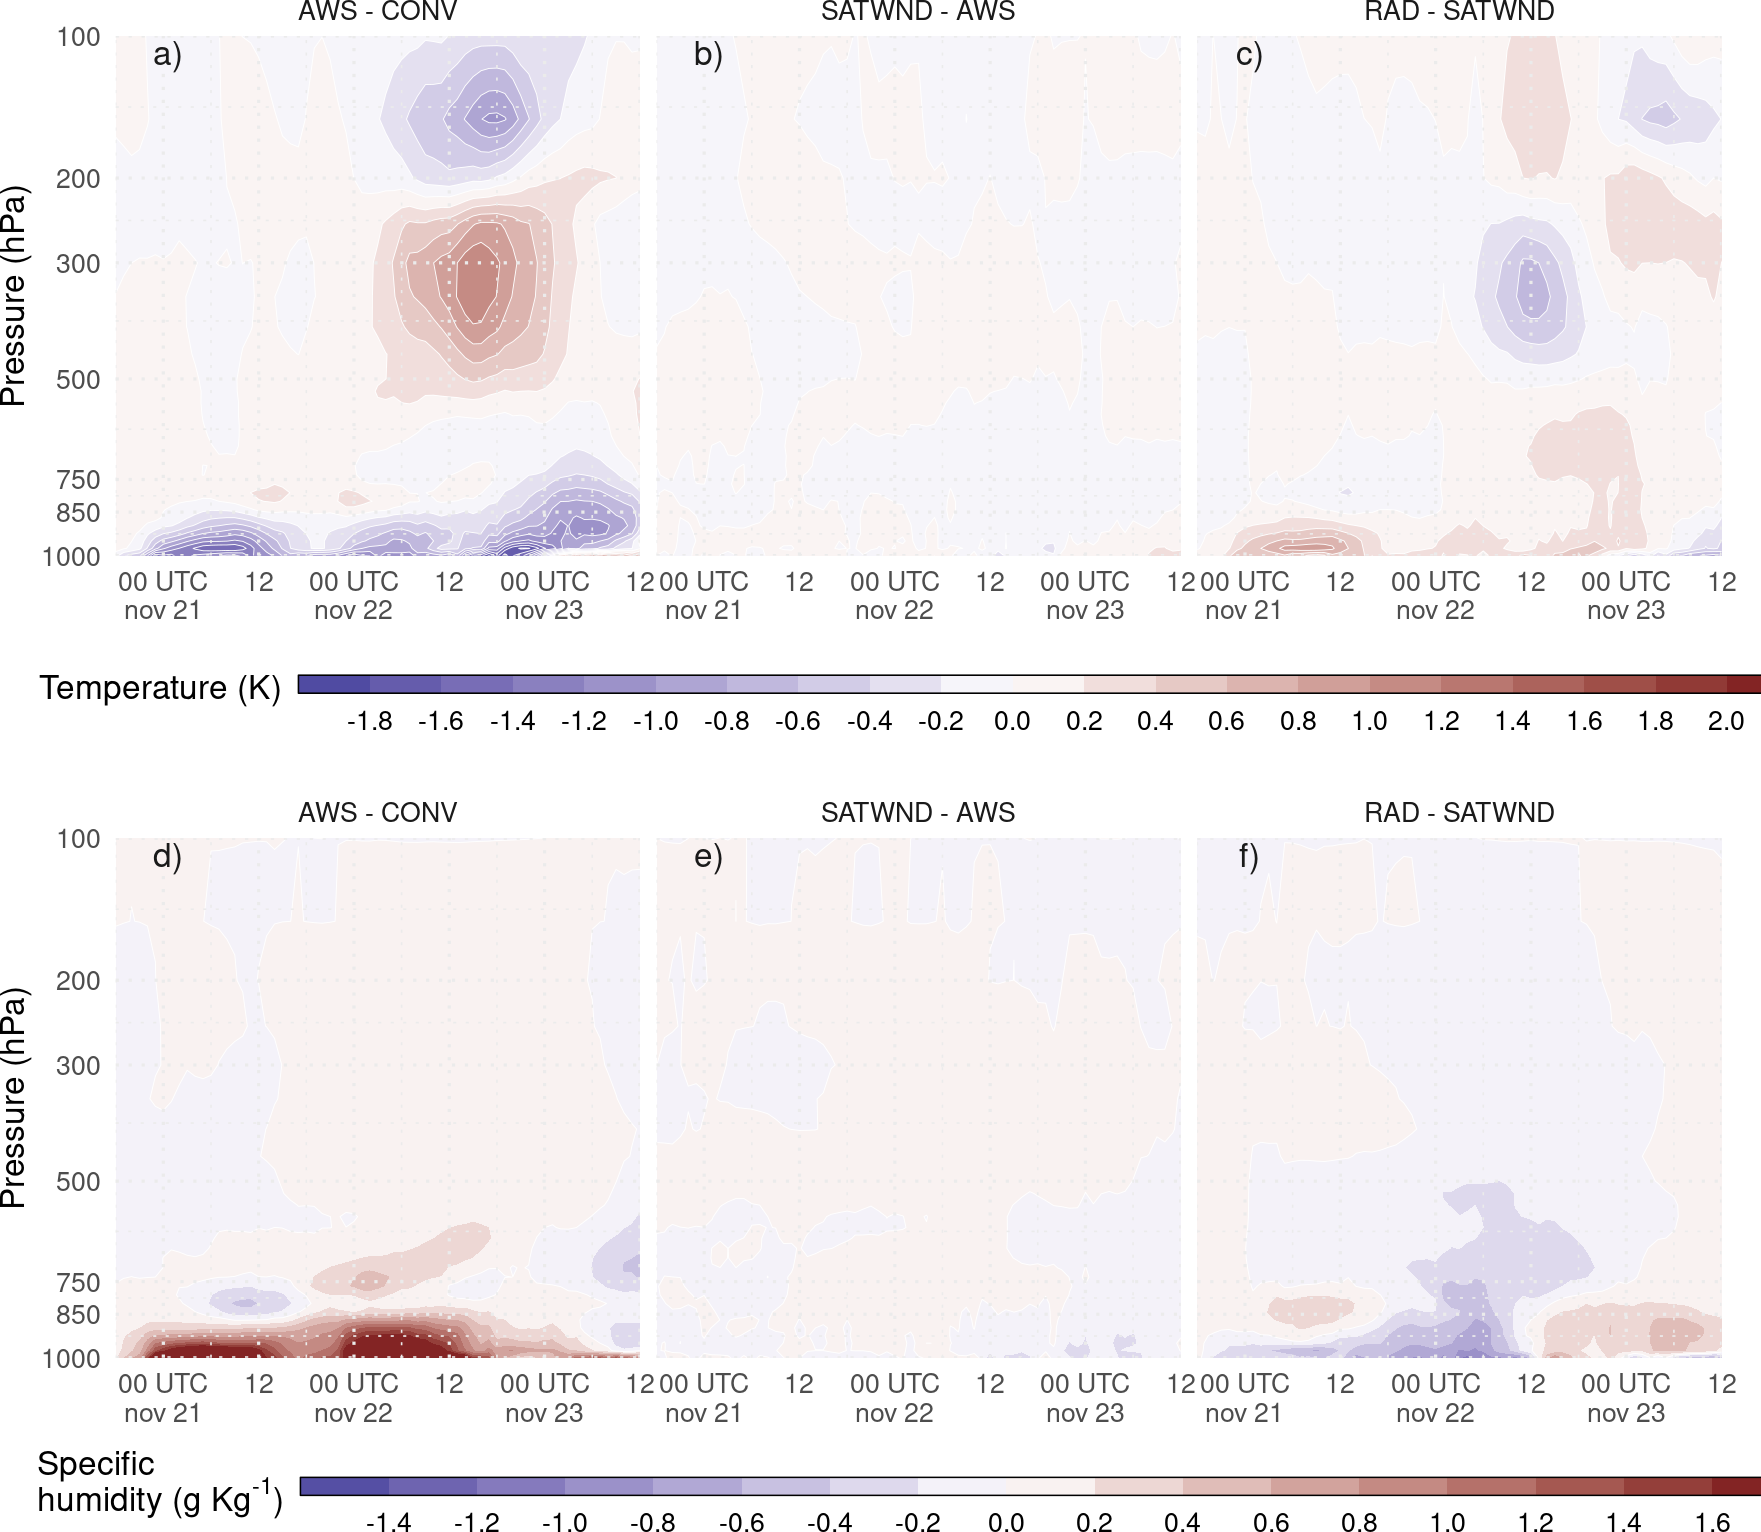
\includegraphics{../figures/TQ-diff-1} 

}

\caption{Difference between experiments AUT-CONV (a and d), SATWND-AUT (b and e) and RAD-SATWND (c and f) for the spatially averaged vertical profiles of temperature (a, b, and c, in \(K\)) and specific humidity (d, e, and f in \(gkg^{-1}\)) calculated over the inner domain (red box in Figure \ref{fig:dominio}a).}\label{fig:TQ-diff}
\end{figure*}



\begin{figure*}[th]

{\centering 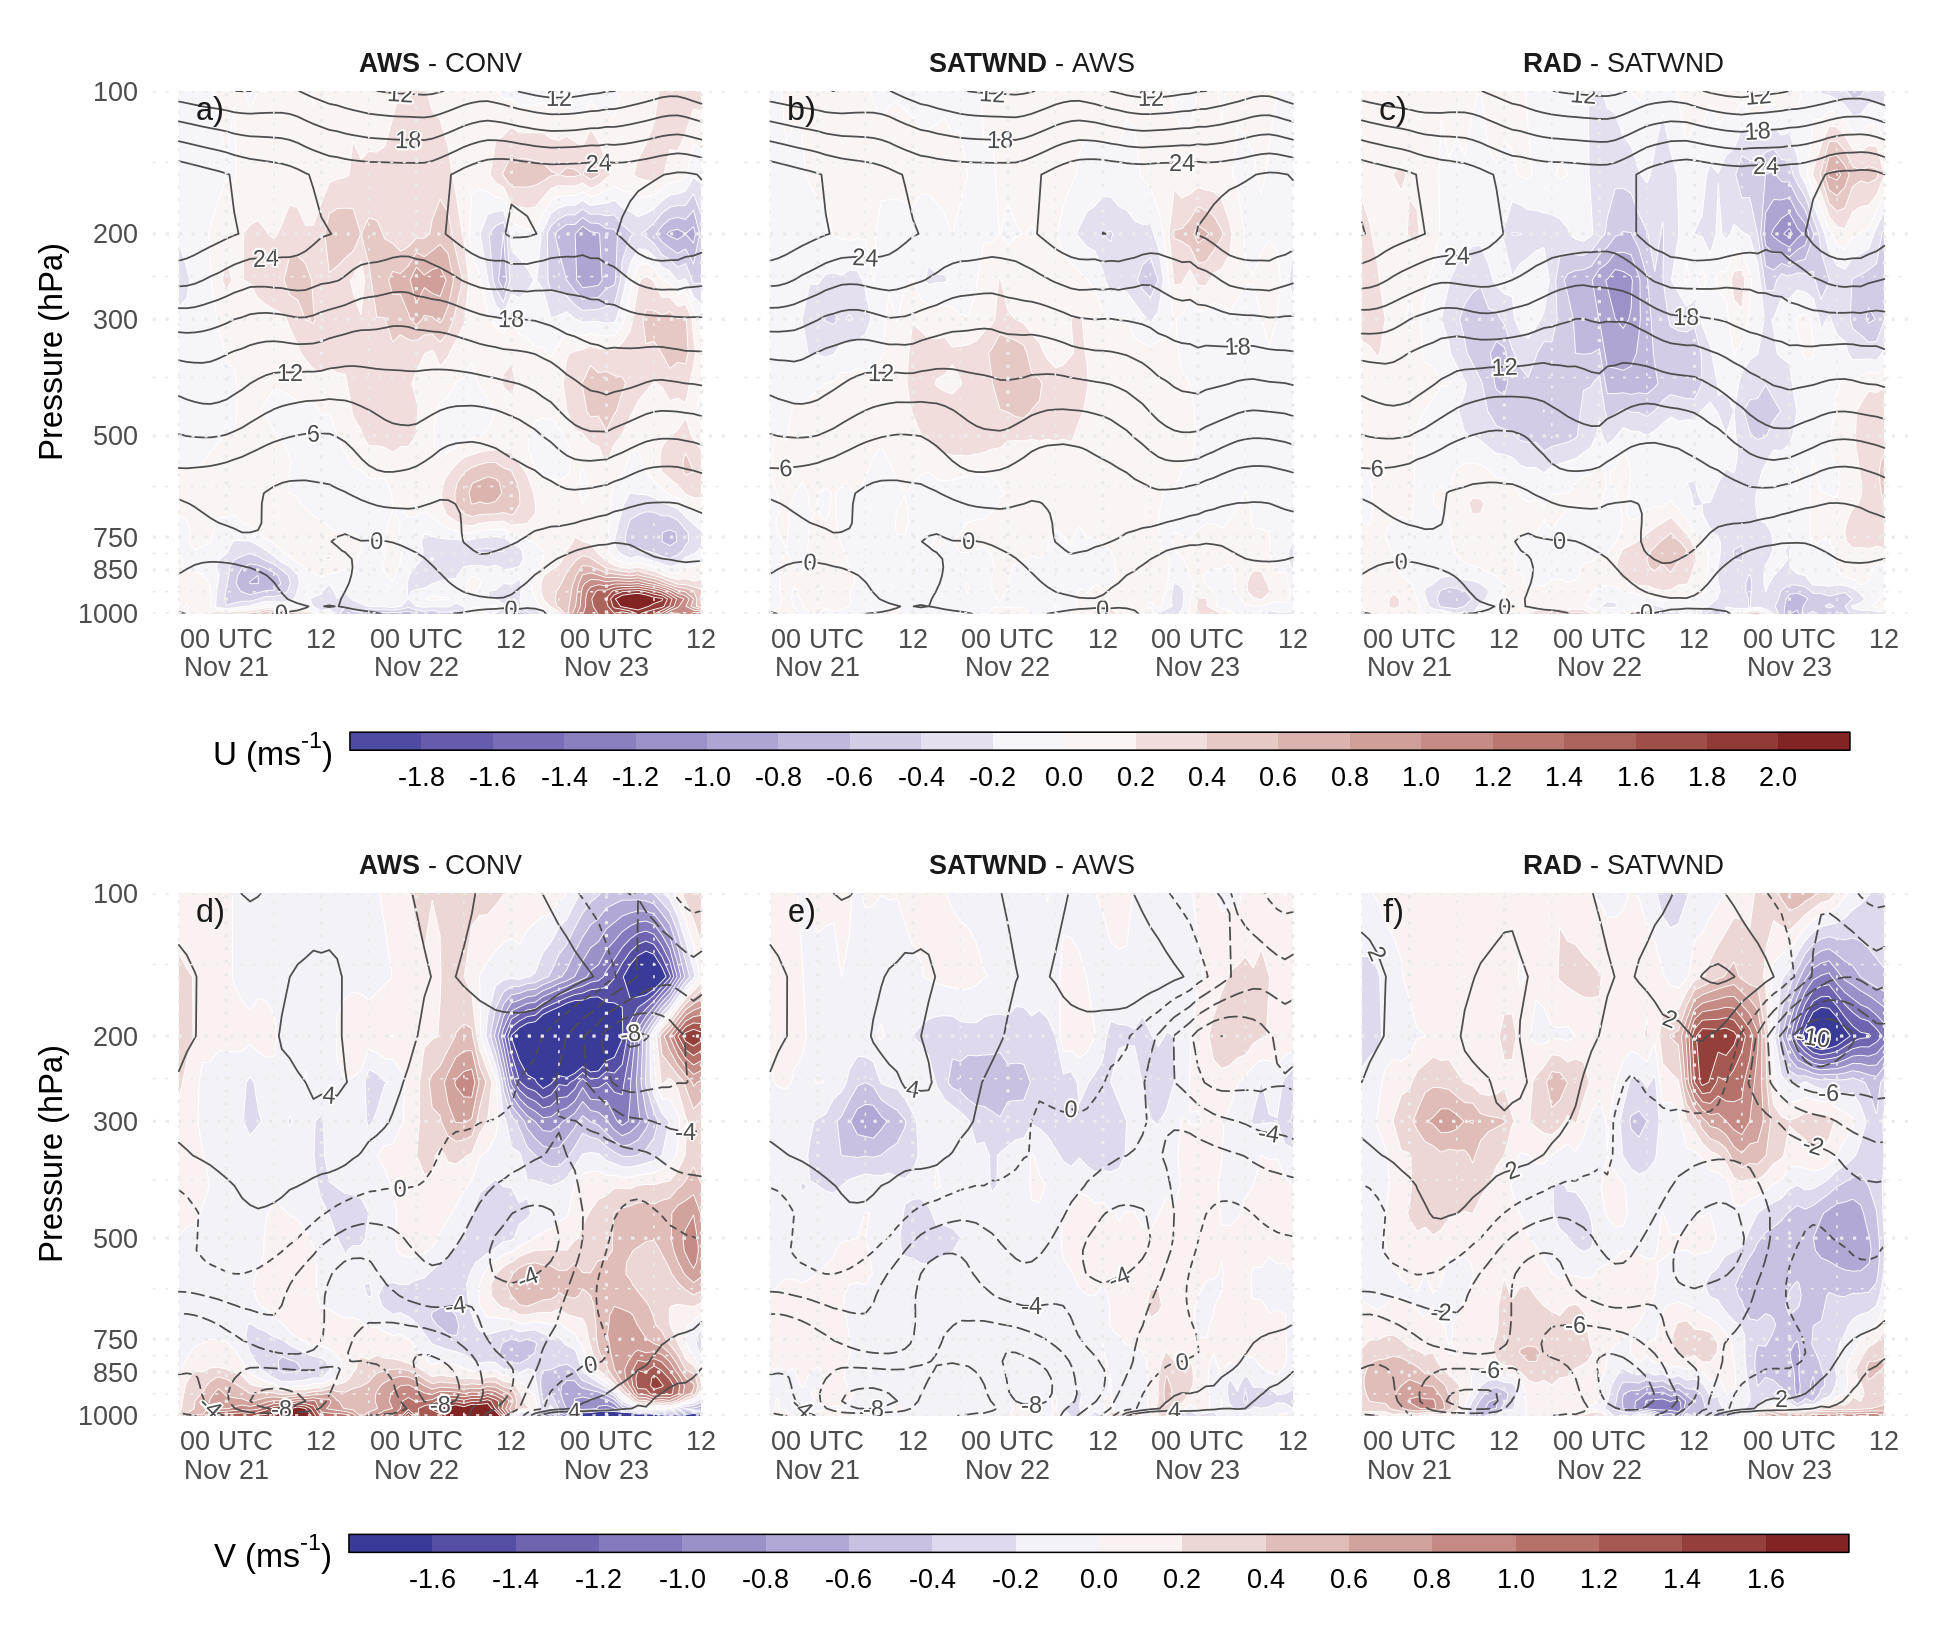
\includegraphics{../figures/UV-diff-1} 

}

\caption{Difference between experiments AUT-CONV (a and d), SATWND-AUT (b and e) and RAD-SATWND (c and f) for the spatially averaged vertical profiles of u wind (a, b, and c, in \(ms^{-1}\)) and v wind (d, e, and f in \(ms^{-1}\)) calculated over the inner domain (red box in Figure \ref{fig:dominio}a). In contours the u wind for AUT (a), SATWND (b) and RAD (c) and v wind for AUT (d), SATWND (e) and RAD (f) are shown.}\label{fig:UV-diff}
\end{figure*}



\begin{figure*}
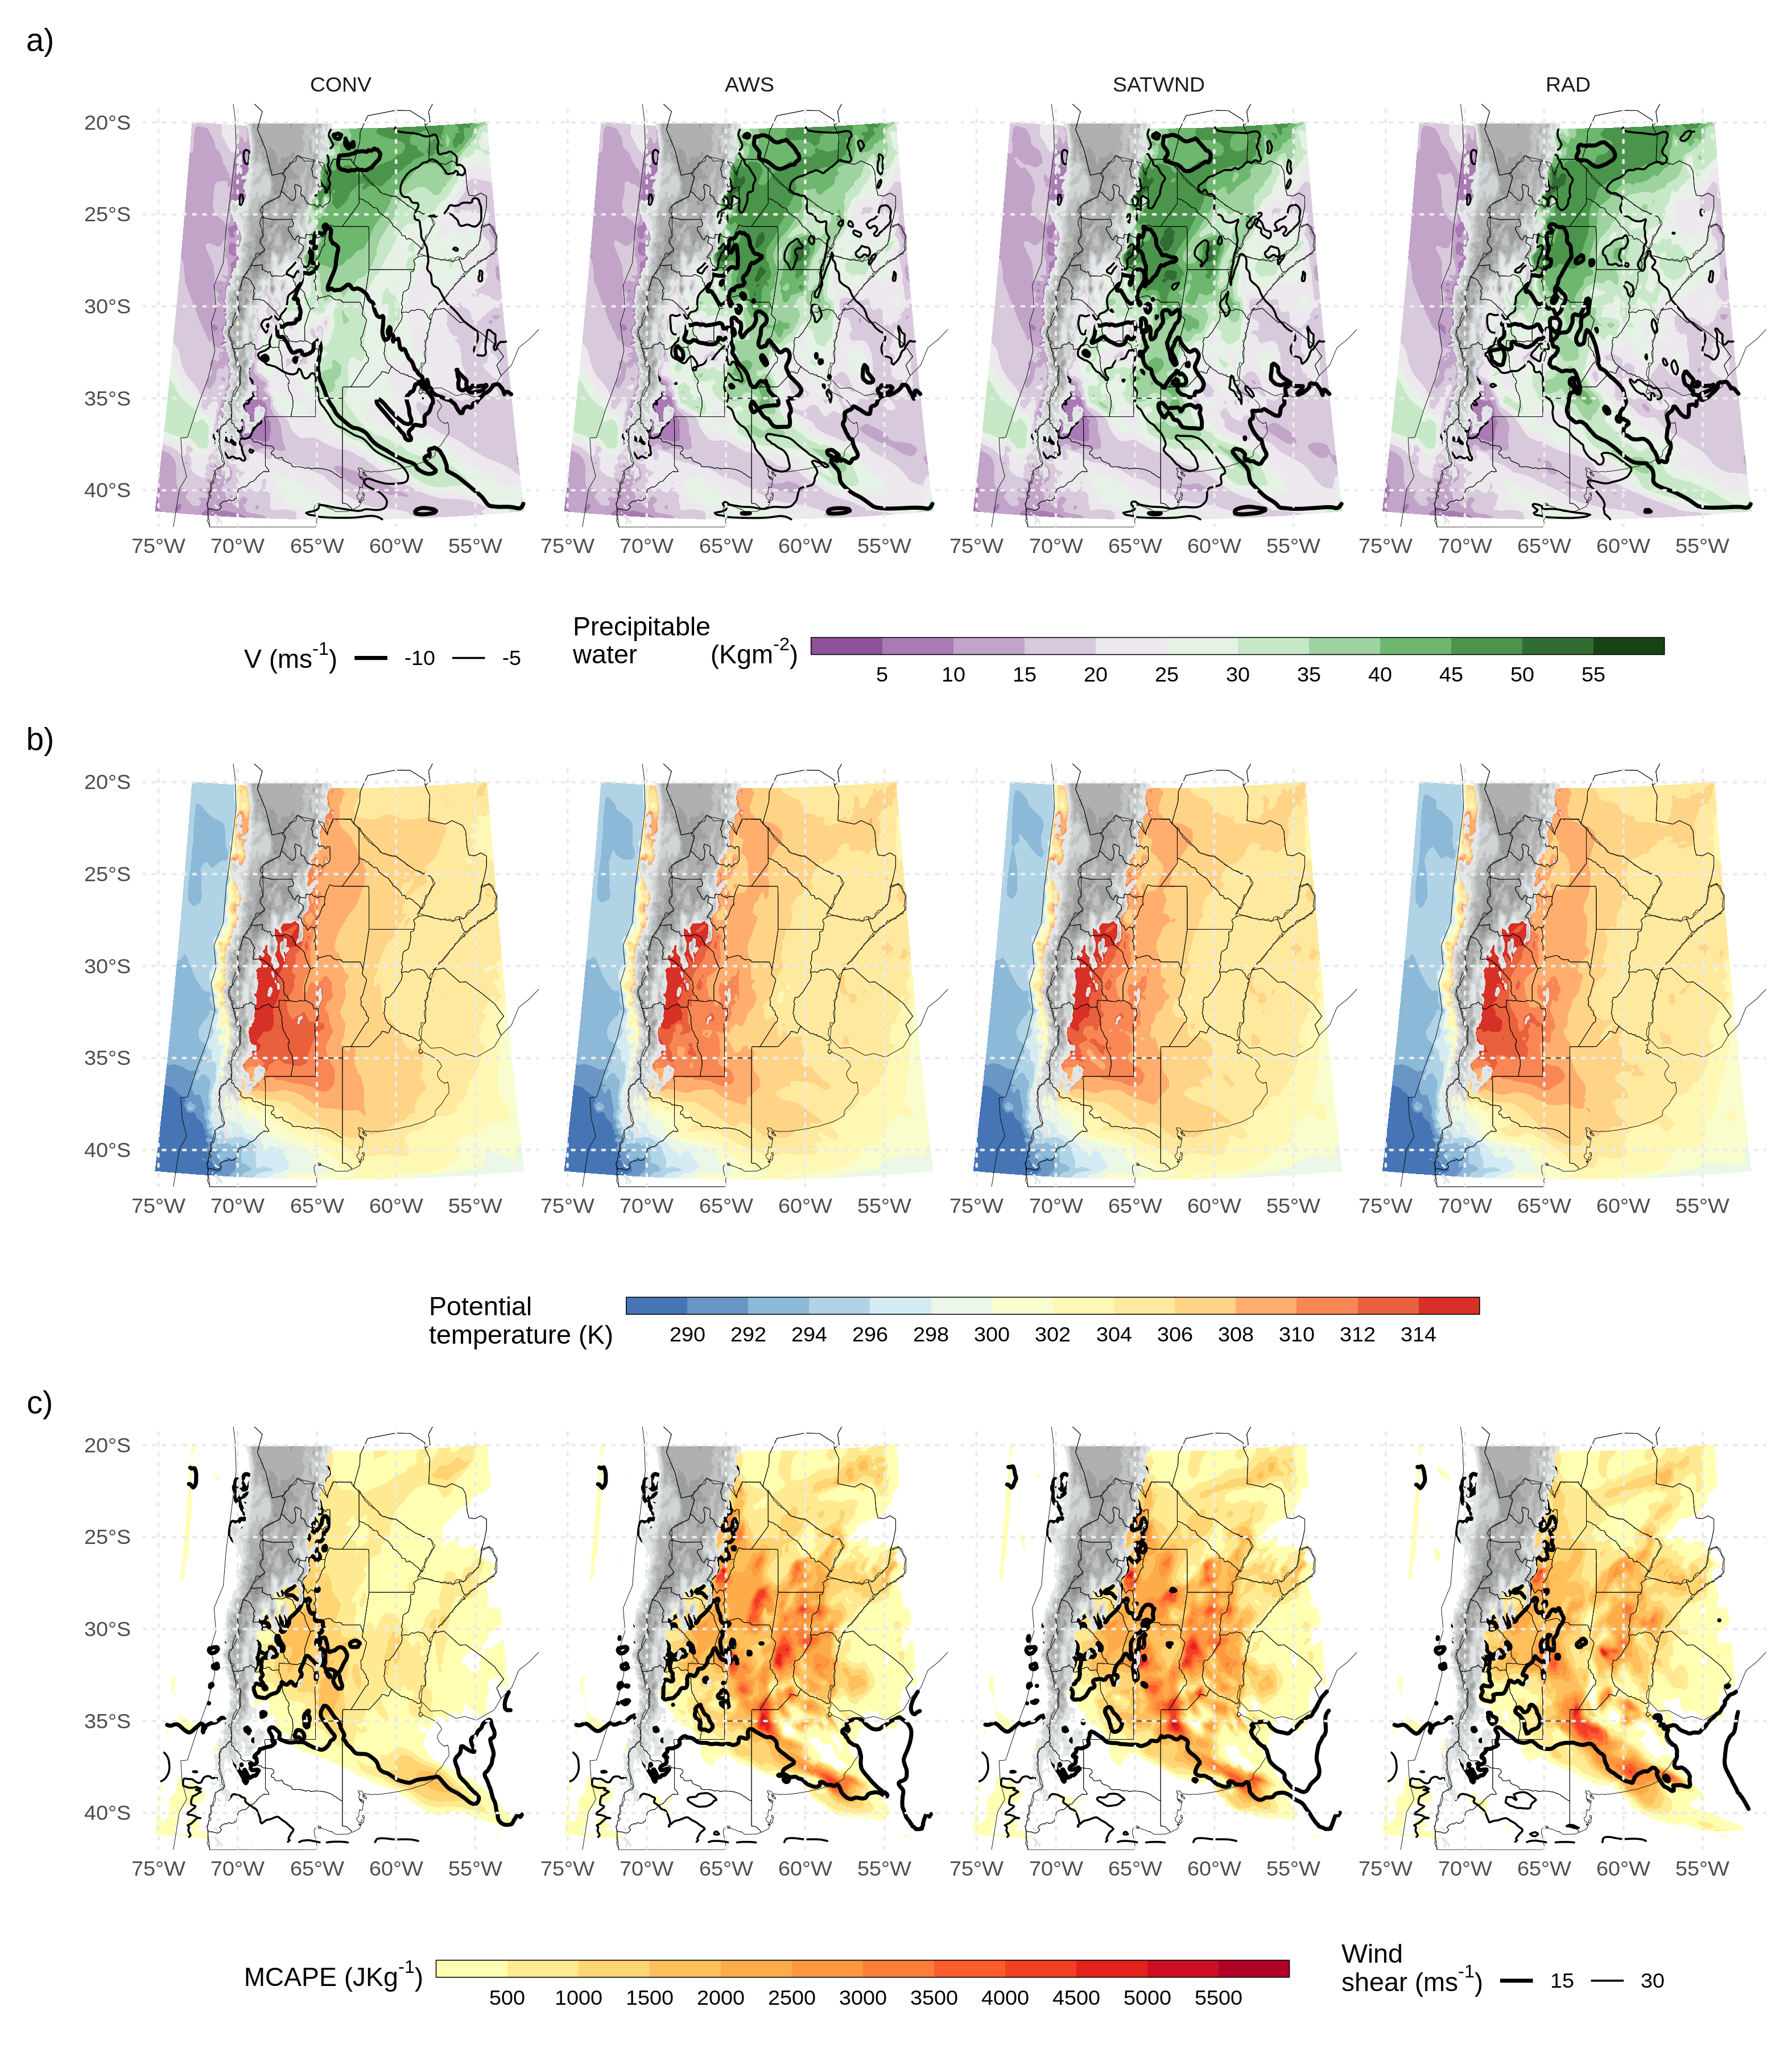
\includegraphics[width=1\linewidth]{../figures/summary-fields-1} \caption{a) Precipitable water (shaded, \(kgm^{-2}\)) and average northerly wind on the first 7 sigma levels (from the surface and up to approximately 800 hPa, contours, \(ms^{-1}\)), b) Average potential temperature for the PBL (first 10 sigma levels) and c) Maximum CAPE and \textasciitilde0-6 km wind shear over 15 and 30 \(ms^{-1}\) for each experiment. All fields correspond to 00 UTC Nov, 22.}\label{fig:summary-fields}
\end{figure*}

\hypertarget{validation-against-independent-observations}{%
\subsection{Validation against independent observations}\label{validation-against-independent-observations}}

Firstly we analyze the impact of different observation types in terms of the representation of the MCS and its associated precipitation. Figure \ref{fig:pp-hov} shows the first-guess hourly accumulated precipitation averaged over a longitude range between 67\(^{\circ}\)W and 54.5\(^{\circ}\)W as a function of time and latitude in the different experiments, and the estimated precipitation by IMERG. The heaviest precipitation (over 12 \(mmh^{-1}\)) starts during the afternoon of Nov 22 and continues during Nov 23 after the end of the simulated period. In all the experiments, the accumulated precipitation in the short-range forecasts underestimates the precipitation. This is particularly evident on CONV where the convection initiation is significantly delayed and occurs further north with respect to the observed initiation. AUT, SATWND, and RAD better capture the timing and location of convective initiation. On RAD the initiation is delayed when we compare with AUT and SATWND possibly due to the lower content of precipitable water and MCAPE on the southern tip of the moist tongue. After 18 UTC Nov, 22 RAD shows improvements in the precipitation rate and its distribution compared to the other experiments as a result of the enhanced development of the convection.



\begin{figure*}[h]
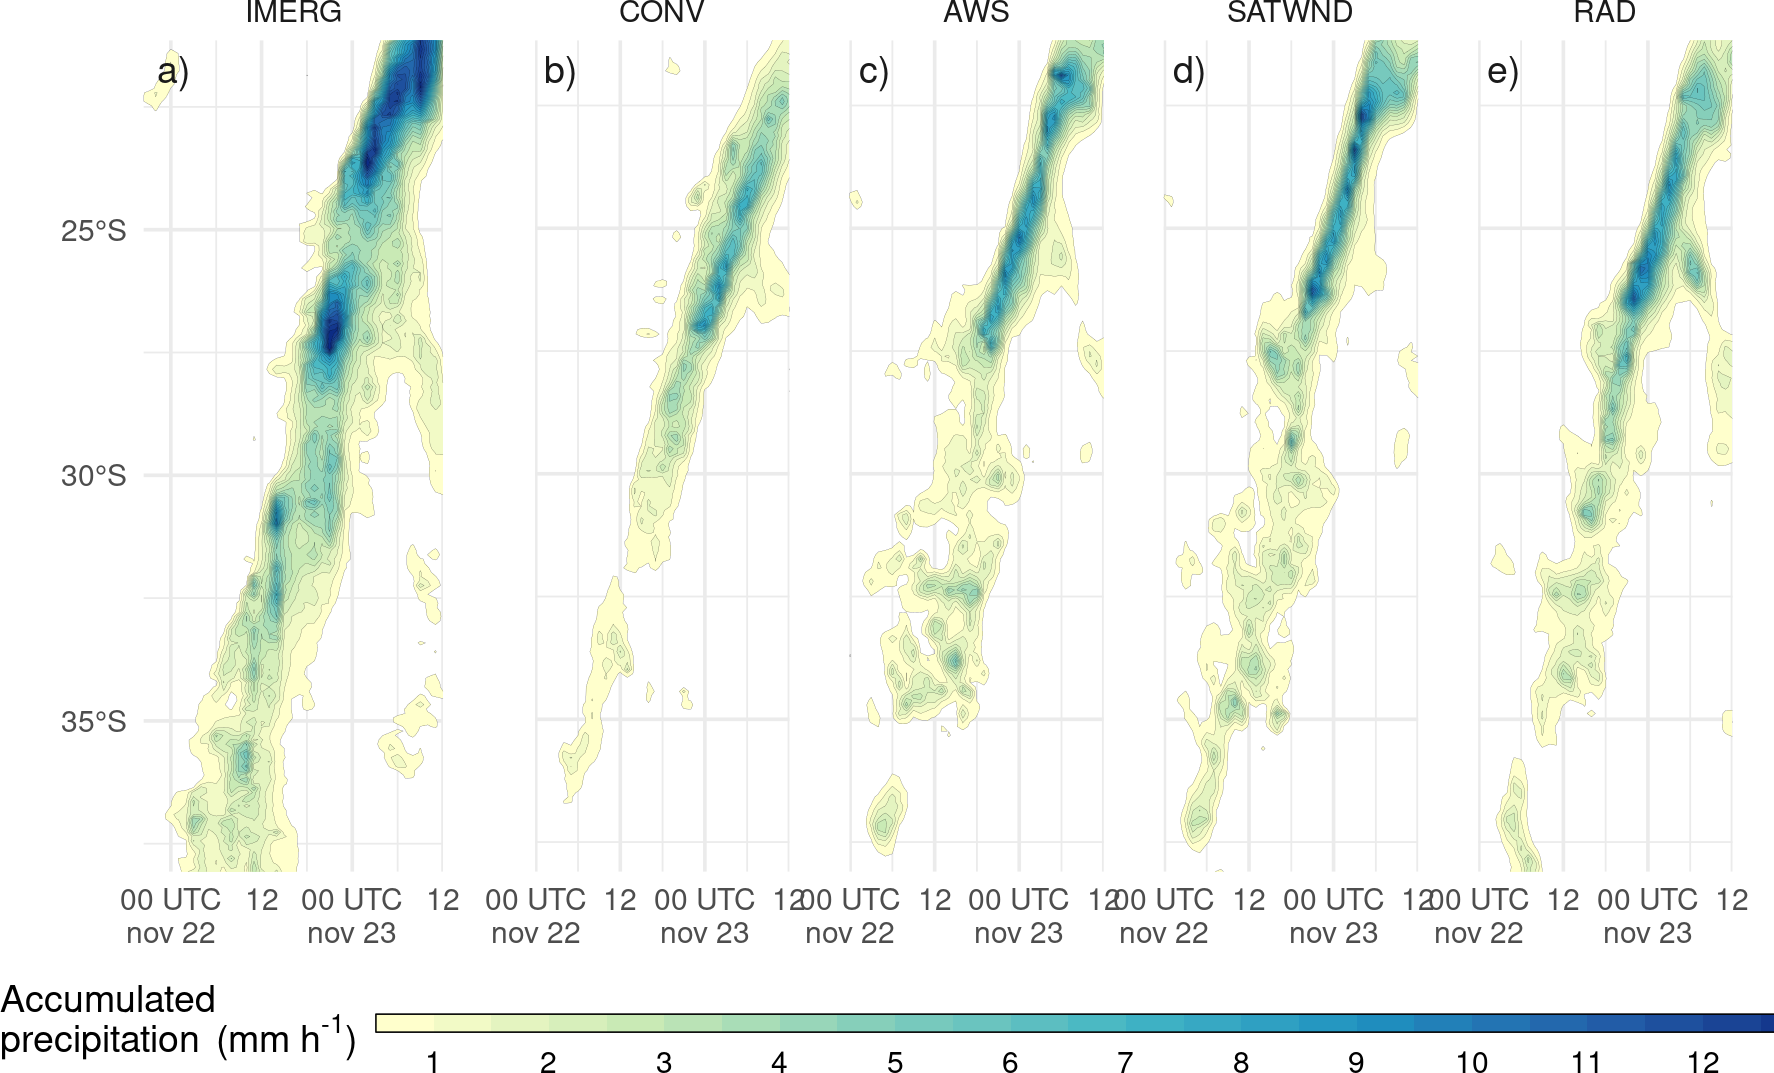
\includegraphics{../figures/pp-hov-1} \caption{Hövmoller of mean hourly accumulated precipitation for each latitude band observed (left) and simulated (right), for the ensemble mean of each experiment, averaged over the inner domain (red box in Figure \ref{fig:dominio}a). Contours drawn every 0.5 \(mmh^{-1}\), starting at 0.5 \(mmh^{-1}\).}\label{fig:pp-hov}
\end{figure*}

To quantify the spatial match between the observed precipitation and the short-range forecasted precipitation for the different experiments, we compute the FSS in 6-hours moving windows for different thresholds and spatial scales (Figure \ref{fig:fss}). All experiments show low values of FSS before and during the initiation of the MCS around 03 UTC Nov, 22, with an improvement during the mature stage of the MCS. The FSS for CONV is the lowest compared to the rest of the experiments and the differences are larger during the mature stage of the MCS. AUT and SATWND show similar FSSs indicating that satellite-derived wind assimilation has little impact on the precipitation for the present case study. The assimilation of radiances led to an overall improvement of the 1-hour forecasted precipitation, particularly for the 25 mm threshold during the period of heaviest precipitation on Nov, 22. The enhancement is also important at the developing stage of the MCS (between 00 and 12 UTC Nov, 22 and for spatial scales above 500 km, not shown).



\begin{figure}
\centering
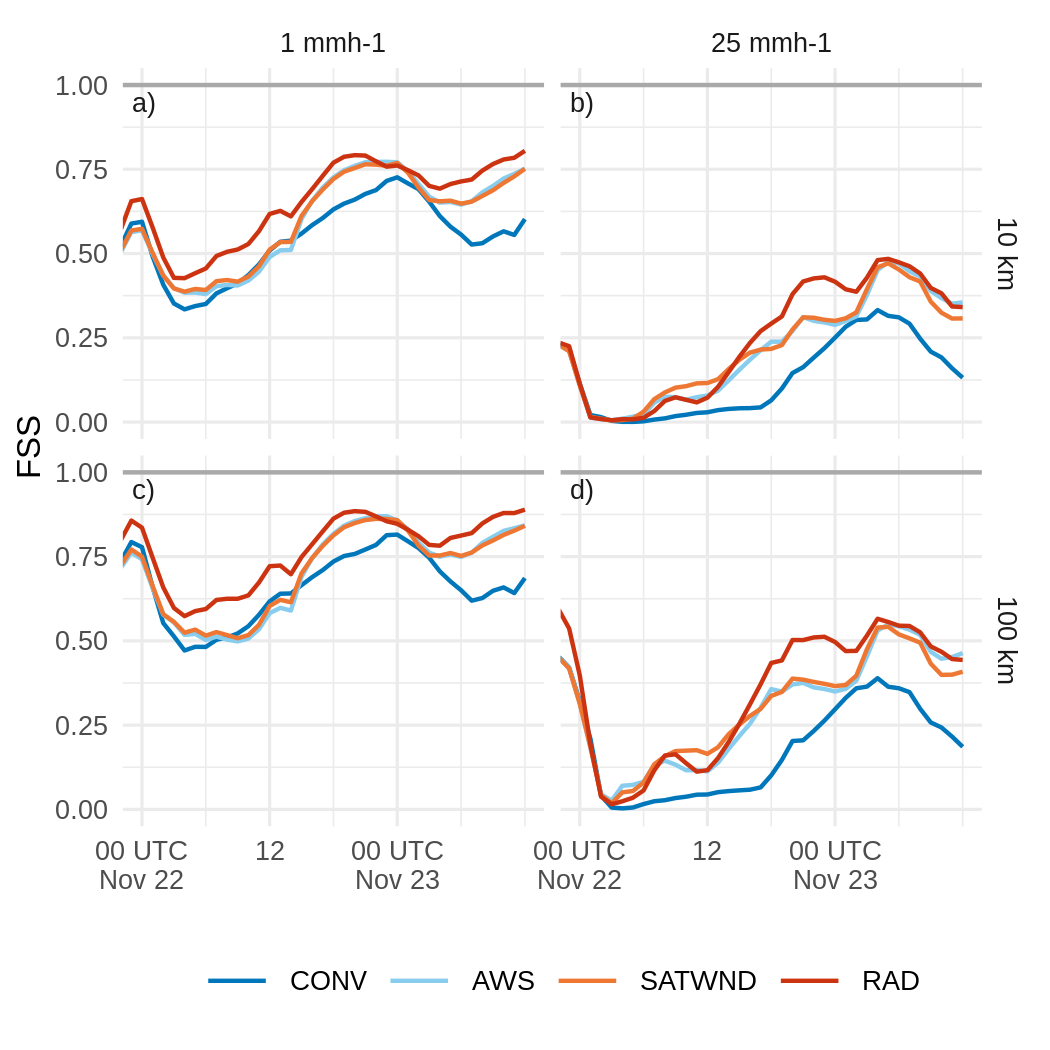
\includegraphics{../figures/fss-1.png}
\caption{\label{fig:fss}FSS calculated over a 6-hours moving window for a) 1 mm and b) 25 mm on a 10 km and c) 1 mm and a d) 25 mm on a 100 km scale, for the CONV (blue line), AUT (ligh blue line), SATWND (orange line) and RAD (red line) experiments.}
\end{figure}

To complement the analysis, Figure \ref{fig:dbz-mean} shows the maximum reflectivity in the column (COLMAX) for the CONV and RAD experiments ensemble mean at different times between 10 and 19 UTC Nov, 22th along with the observed maximum reflectivity. These experiments were chosen because they represent the analysis with the minimum and the maximum number of assimilated observations. In addition, these experiments are the worst and best performing experiments in terms of the short-range precipitation forecast skill. Overall none of the short-range forecasts is able to capture the mesoscale details in the precipitation distribution. This is partially expected considering the relatively low horizontal resolution (10 km) which is not enough to appropriately capture the strength of the convective band associated with the MCS. Also, the ensemble mean produces a smoothing effect that reduces the amplitude of local maxima in the forecasted reflectivity field. RAD better represents the observed features of the MSC showing a more strong and organized MCS over the domain center at 10 and 13 UTC (first and second columns in Figure \ref{fig:dbz-mean}). The convective cells that initiate after 16 UTC over the warm front in the northeast part of the domain are well captured by both experiments, but better represented in terms of strength in the RAD experiment. CONV captures the location of the MCS, but the convection seems to be less organized and much weaker than in RAD. Before and after the times shown in Figure \ref{fig:dbz-mean}, the agreement between experiment and observations is quite high in the regions where radar data are available.

Finally, Figure \ref{fig:soundings} shows the RMSE and bias calculated by comparing the experiments with radiosonde data from the RELAMPAGO missions, IOP 7 from 15 to 21 UTC Nov, 21 (including 30 radiosondes) and IOP 8 from 14 to 20 UTC Nov 22 (including 22 radiosondes). IOP 7 provides a good characterization of the pre-convective environment during the first day of our experiments. The area where the observations were taken was characterized by mostly clear skies and a low-level northerly flow associated with warm and moist advection. For the temperature, CONV presents a warm bias on the PBL of 1\(^{\circ}\)C and an RMSE between 1 and 2.5\(^{\circ}\)C that is slightly reduced by the assimilation of ASWS and radiances. The RMSE for temperature remains between 0.5 and 2\(^{\circ}\)C throughout the troposphere and lower stratosphere and the impact of additional observations in the AUT, SATWND, and RAD is small above the PBL. The dew point temperature shows a small dry bias in low levels that is corrected on AUT, SATWND, and RAD. On middle levels (below 10 km) the bias is large and positive (8 - 10\(^{\circ}\)C), indicating a more moist atmosphere in the analysis. Overall, the RMSE grows with height, this is probably because at upper levels, moisture contents are lower and small changes in the amount of water vapor can produce relatively large differences in terms of dew point temperatures. The zonal wind has a significant positive bias of approximately 10 \(ms^{-1}\) in the upper troposphere which is mainly reduced by assimilating satellite radiances. It is somewhat surprising that no significant effect is observed by assimilating satellite-derived winds. The assimilation of ASWS and radiance observations increases the northerly wind bias and RMSE near the surface.



\begin{figure*}[h]
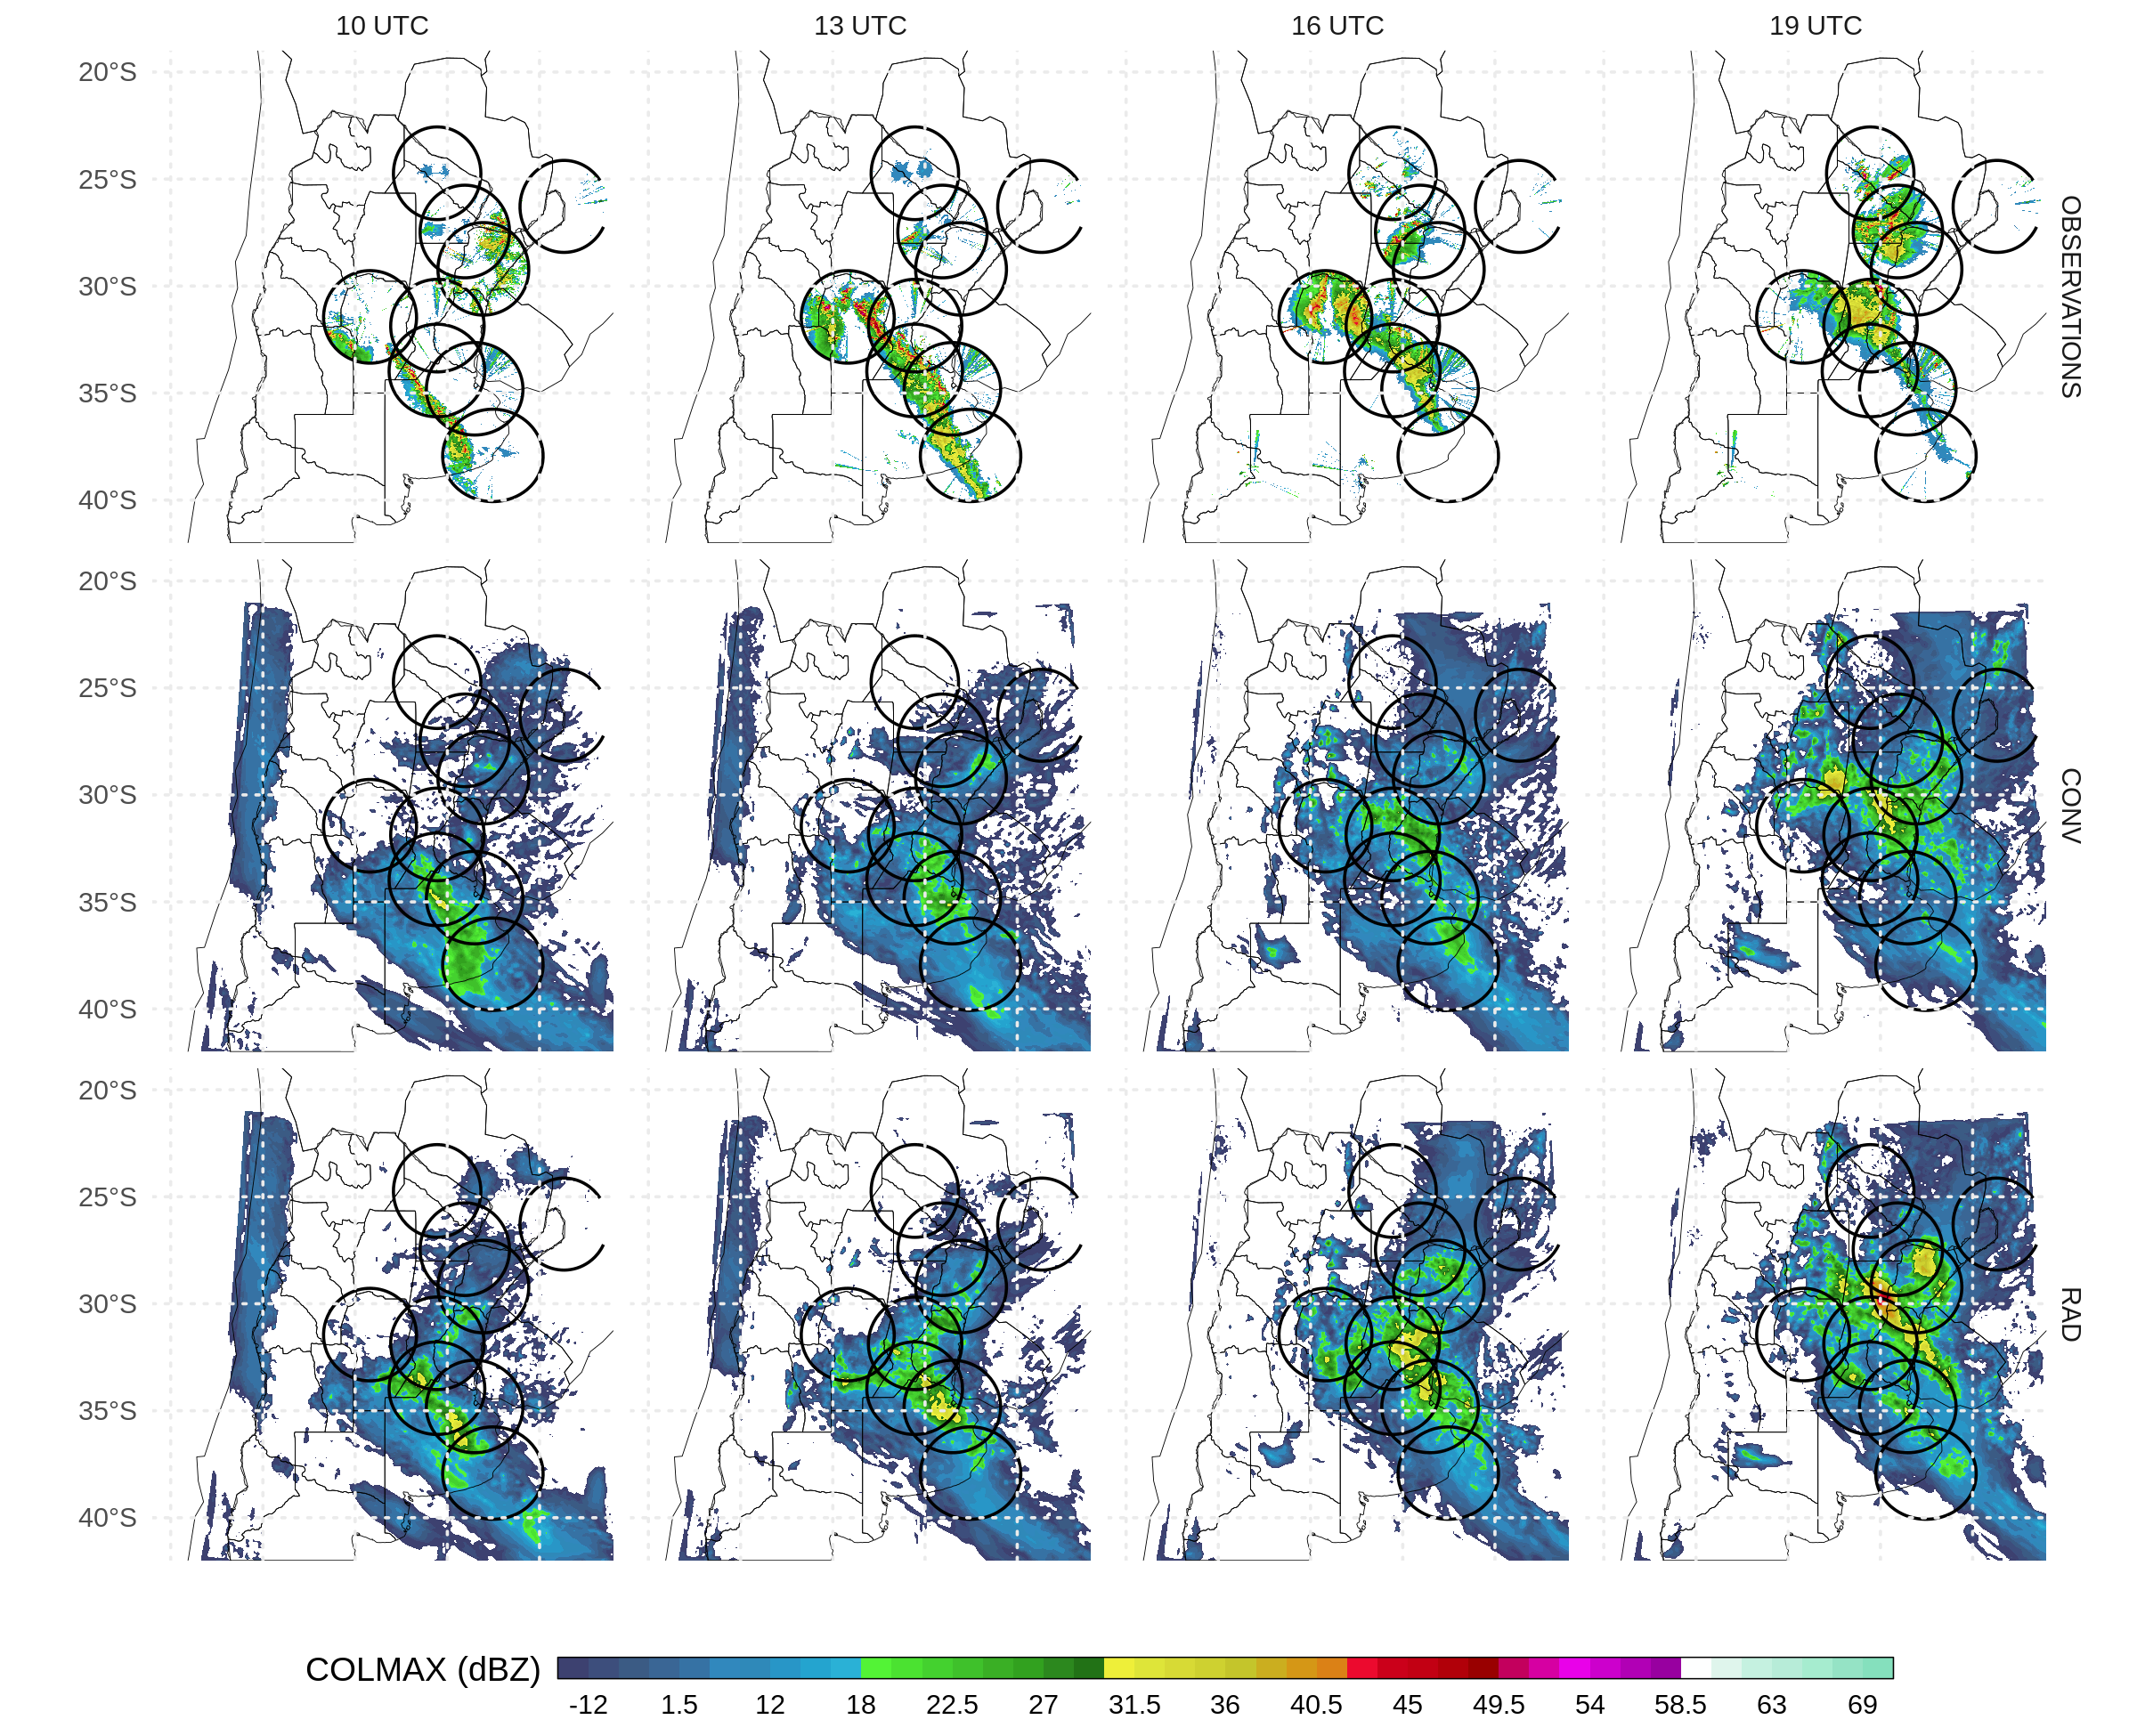
\includegraphics[width=1\linewidth]{../figures/dbz-mean-1} \caption{Observed maximum reflectivity in the column (upper row) and 1-hr forecasted ensemble mean maximum reflectivity for CONV (second row) and RAD (third rows) at 10 UTC (first column), 13 UTC (second column), 16 UTC (third column), and 19 UTC (fourth column) Nov, 22.}\label{fig:dbz-mean}
\end{figure*}

For the IOP 8 (bottom row in Figure \ref{fig:soundings}), the densely observed area was behind the MCS, but far enough from it to be directly affected by its mesoscale circulations. This area was also behind the cold front thus affected by low-level cold advection. Below 5km all experiments show a warm bias which decreases with the assimilation of ASWS and radiances. Between 5 and 12 km, the bias in each experiment is cold and is reduced in AUT, SATWND, and RAD to the assimilations of ASWS. The RMSE for AUT, SATWND, and RAD remains below 2\(^{\circ}\)C for almost all levels with significant improvement in upper levels where radiance observations have the largest impact. In terms of the dew point temperature, the analyses have a moist bias near the surface that increases with the incorporation of new observations. This moist bias is mostly driven by the assimilation of surface temperature observations and the fact that near the surface there is a negative covariance between temperature and moisture content over this region. The reason why such a covariance structure emerges from the ensemble is not clear and deserves further investigation but it is evident that the corrections introduced by the observations are degrading the estimation of the moisture content within the PBL. SATWND presents the lowest RMSE overall while AUT and RAD are comparable between 4 and 12 km with values that do not exceed 7\(^{\circ}\)C. The zonal wind is overestimated on the analyses with a positive bias at middle levels. For this period only RAD shows an improvement in the upper troposphere. At low levels the meridional wind presents a negative bias, indicating an underestimation of the southerly wind behind the cold front principally in AUT, SATWND, and RAD. In fact, low level biases, in these experiments, are higher than in the CONV experiment indicating a detrimental effect of the additional observations (possibly associated with the effect of ASWS).



\begin{figure*}[t]

{\centering 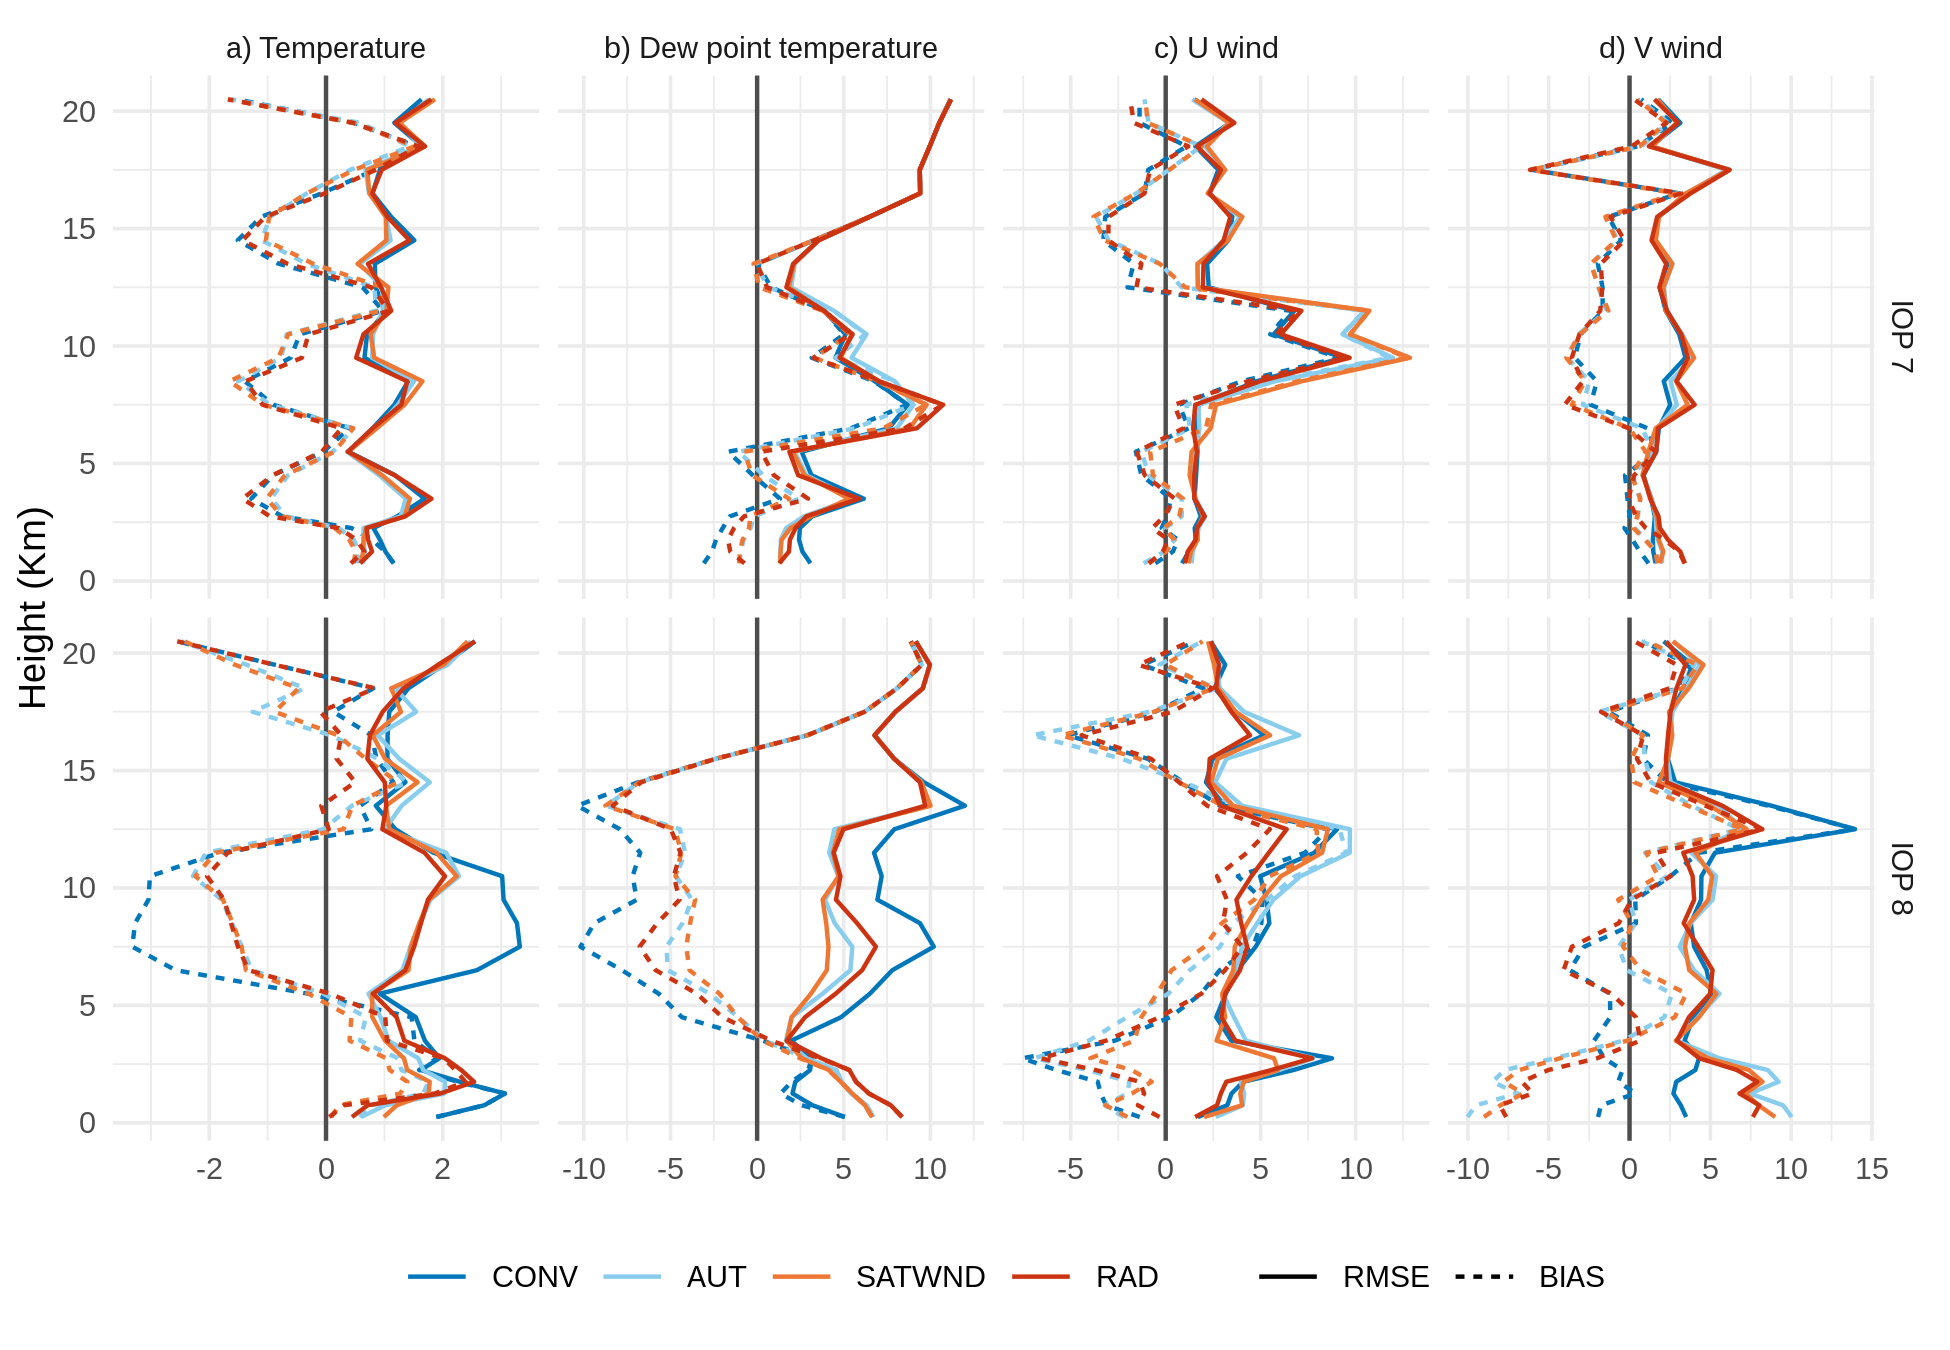
\includegraphics{../figures/soundings-1} 

}

\caption{RMSE (solid line) and Bias (dash line) of a) temperature, b) dew point temperature, c) u wind and d) v wind calculated by comparing each experiment with the RELAMPAGO soundings during IOP 7 and IOP 8. The blue line correspond to CONV, the ligh blue line to AUT, SATWND is represented with an orange line and RAD with a red line.}\label{fig:soundings}
\end{figure*}

\hypertarget{conclusions}{%
\section{Conclusions}\label{conclusions}}

We performed four experiments to assess the impact of different observation types, including frequent surface observations, satellite-derived winds, and clear-sky satellite radiances, into a regional frequent-update ensemble-based data assimilation system. We used a case study approach of a massive MCS developed over Southern South America on Nov 22, 2018.

We evaluated the reliability of the ensemble using the RCRV calculated for each type of observation used in RAD. Conventional observations including surface observation and upper air observations from soundings and aircraft show a \(sd RCRV\) near 1 indicating a good agreement between the ensemble spread and the observational errors with respect to the distance between the ensemble mean and the observations. For satellite-derived winds and radiance observations, the \(sd RCRV\) is lower than 1. This could be the result of an underdispersive ensemble or an overestimation of the observation errors. Taking into account that the errors of this type of observation are usually overestimated to avoid strong impacts on the analysis for poor quality observations and the results obtained for more reliable observations such as soundings, we conclude that the assembly has a reasonable spread.

In terms of the analysis, we found that ASWS observations that have high spatial and temporal resolution produce major impacts throughout the troposphere and mainly on the PBL. In particular, the precipitable water content and the low level meridional circulation lead to the development of deep convection and heavy precipitation closer to the observed in this case study. We also found positive results when assimilating radiance observations that produce a better development of the convection, mainly during the mature state of the MCS leading to an increase in the accumulated precipitation compared with the other experiments. However, all experiments underestimated the 1-hour accumulated precipitation when compared to IMERG estimates. While the assimilation of satellite-derived wind does not impact substantially on the analysis, this is possible due to the small number of observations in low levels available for this case study. A more comprehensive analysis is necessary to assess the possible impacts on middle and upper levels.

Taking advantage of the observations taken during the RELAMPAGO field campaign we compared the experiments with the soundings launched during the IOPs 7 and 8. For the pre-convective environment (IOP 7), we observed an improvement on low level when assimilating ASWS observations on the temperature, dew point temperature, and meridional wind. In particular, ASWS observations correct a dry bias already observed by Ruiz et al. (2010). For IOP 8, after the MCS crossed the center of the domain, we found a positive impact in low levels for the temperature but the opposite effect for the dew point temperature. In this case, the analyses have a moist bias that increases with the assimilation of ASWS and radiances observations. We observed a negative covariance between temperature and moisture content over this region that could lead to a moistening of the PBL. It is not clear what produces these negative covariances but it is evident that the corrections introduced by the observations are degrading the estimation of the moisture content during this period and they require further analysis.

To summarize this study, we conclude that the assimilation of surface observations with higher spatial and temporal resolution and clear-sky radiances from polar orbit satellites had an overly positive impact on the development of the studied MCS and its associated precipitation. In the future, we will analyze whether these impacts carry over in time to the independent forecasts initialized from the analyses.

\hypertarget{acknowledgements}{%
\section{Acknowledgements}\label{acknowledgements}}

We are very thankful to the Atmospheric and Sea Research Center (CIMA), the University of Buenos Aires (UBA) and the National Scientific and Technical Research Council (CONICET) who support this study. We acknowledge the Argentinian National Meteorological Service (ANMS) for kindly providing the radar observations used for validation. We also acknowledge the Cheyenne HPC resources (doi:10.5065/D6RX99HX) from NCAR's Computational and Information Systems Laboratory, National Science Foundation (project code UIUC0012). Also, PICT 2017-2033 and PICT 2016-0710 projects of the National Agency for the Promotion of Research, Technological Development and Innovation from Argentina partially funded this project.

\hypertarget{references}{%
\section*{References}\label{references}}
\addcontentsline{toc}{section}{References}

\hypertarget{refs}{}
\leavevmode\hypertarget{ref-allaire2020}{}%
Allaire, J.J., Xie {[}aut, Y., cre, McPherson, J., Luraschi, J., Ushey, K., Atkins, A., Wickham, H., Cheng, J., Chang, W., Iannone, R., Dunning, A., filter), A.Y.(. sections L., Schloerke, B., Dervieux, C., Aust, F., Allen, J., Seo, J., Barrett, M., Hyndman, R., Lesur, R., Storey, R., Arslan, R., Oller, S., RStudio, PBC, library), j.F.(., inst/rmd/h/jquery-AUTHORS.txt), j. contributors (. library; authors listed in, inst/rmd/h/jqueryui-AUTHORS.txt), j.U. contributors (.U. library; authors listed in, library), M.O.(., library), J.T.(., library), B. contributors (., Twitter, library), I.(., library), A.F.(., library), S.J.(. js, library), I.S.(. js, library), G.F.(., templates), J.M.(., Google, library), I.(., library), D.R.(., library), W.(., Gandy (Font-Awesome), D., Sperry (Ionicons), B., (Ionicons), D., StickyTabs), A.L.(., filter), B.P.J.(.L., filter), A.K.(.L., 2020. Rmarkdown: Dynamic Documents for R.

\leavevmode\hypertarget{ref-bao2015}{}%
Bao, Y., Xu, J., Powell Jr., A.M., Shao, M., Min, J., Pan, Y., 2015. Impacts of AMSU-A, MHS and IASI data assimilation on temperature and humidity forecasts with GSI--WRF over the western United States. Atmos. Meas. Tech. 8, 4231--4242. doi:\href{https://doi.org/10.5194/amt-8-4231-2015}{10.5194/amt-8-4231-2015}

\leavevmode\hypertarget{ref-brooks2003}{}%
Brooks, H.E., Lee, J.W., Craven, J.P., 2003. The spatial distribution of severe thunderstorm and tornado environments from global reanalysis data. Atmospheric Research 67-68, 73--94. doi:\href{https://doi.org/10.1016/S0169-8095(03)00045-0}{10.1016/S0169-8095(03)00045-0}

\leavevmode\hypertarget{ref-campitelli2020}{}%
Campitelli, E., 2020. metR: Tools for Easier Analysis of Meteorological Fields.

\leavevmode\hypertarget{ref-candille2007}{}%
Candille, G., Côté, C., Houtekamer, P.L., Pellerin, G., 2007. Verification of an Ensemble Prediction System against Observations. Mon. Wea. Rev. 135, 2688--2699. doi:\href{https://doi.org/10.1175/MWR3414.1}{10.1175/MWR3414.1}

\leavevmode\hypertarget{ref-cecil2012}{}%
Cecil, D.J., Blankenship, C.B., 2012. Toward a Global Climatology of Severe Hailstorms as Estimated by Satellite Passive Microwave Imagers. Journal of Climate 25, 687--703. doi:\href{https://doi.org/10.1175/JCLI-D-11-00130.1}{10.1175/JCLI-D-11-00130.1}

\leavevmode\hypertarget{ref-chen2001}{}%
Chen, F., Dudhia, J., 2001. Coupling an Advanced Land Surface--Hydrology Model with the Penn State--NCAR MM5 Modeling System. Part I: Model Implementation and Sensitivity. Monthly Weather Review 129, 569--585. doi:\href{https://doi.org/10.1175/1520-0493(2001)129\%3C0569:CAALSH\%3E2.0.CO;2}{10.1175/1520-0493(2001)129\textless0569:CAALSH\textgreater2.0.CO;2}

\leavevmode\hypertarget{ref-chen2015}{}%
Chen, Q., Fan, J., Hagos, S., Gustafson, W.I., Berg, L.K., 2015. Roles of wind shear at different vertical levels: Cloud system organization and properties. Journal of Geophysical Research: Atmospheres 120, 6551--6574. doi:\href{https://doi.org/10.1002/2015JD023253}{10.1002/2015JD023253}

\leavevmode\hypertarget{ref-Cheyenne2019}{}%
Computational and Information Systems Laboratory, 2019. Cheyenne: HPE/SGI ICE XA System (University Community Computing). National Center for Atmospheric Research Boulder, CO. doi:\href{https://doi.org/doi:10.5065/D6RX99HX}{doi:10.5065/D6RX99HX}

\leavevmode\hypertarget{ref-deelia2017}{}%
de Elía, R., Vidal, L., Lohigorry, P., 2017. El SMN y la red argentina de radares meteorológicos {[}WWW Document{]}. URL \url{http://hdl.handle.net/20.500.12160/625}

\leavevmode\hypertarget{ref-dillon2019}{}%
Dillon, M.E., García Skabar, Y., Kalnay, E., Ruiz, J.J., Collini, E.A., 2019. Sensibilidad de un sistema de asimilación de datos por ensambles a diferentes configuraciones, implementado en el sur de Sudamérica. Meteorológica 44, 15--34.

\leavevmode\hypertarget{ref-dillonInreview}{}%
Dillon, M.E., Maldonado, P., Corrales, P., García Skabar, Y., Ruiz, J.J., Sacco, M., Cutraro, F., Mingari, L., Matsudo, C., Vidal, L., Rugna, M., Hobouchian, M.P., Salio, P., Nesbitt, S., Saulo, C., Kalnay, E., Miyoshi, T., n.d. A Rapid Refresh ensemble based Data Assimilation and Forecast system for the RELAMPAGO field campaign. Atmospheric Research.

\leavevmode\hypertarget{ref-dillon2016}{}%
Dillon, M.E., Skabar, Y.G., Ruiz, J., Kalnay, E., Collini, E.A., Echevarría, P., Saucedo, M., Miyoshi, T., Kunii, M., 2016. Application of the WRF-LETKF Data Assimilation System over Southern South America: Sensitivity to Model Physics. Wea. Forecasting 31, 217--236. doi:\href{https://doi.org/10.1175/WAF-D-14-00157.1}{10.1175/WAF-D-14-00157.1}

\leavevmode\hypertarget{ref-dowle2020}{}%
Dowle, M., Srinivasan, A., 2020. Data.Table: Extension of 'data.frame'.

\leavevmode\hypertarget{ref-sondeos}{}%
Earth Observing Laboratory, U. -, 2020. Multi-network composite highest resolution radiosonde data. Version 1.3. UCAR/NCAR - earth observing laboratory.

\leavevmode\hypertarget{ref-gao2015}{}%
Gao, F., Huang, X.-Y., Jacobs, N.A., Wang, H., 2015. Assimilation of wind speed and direction observations: Results from real observation experiments. Tellus A: Dynamic Meteorology and Oceanography 67, 27132. doi:\href{https://doi.org/10.3402/tellusa.v67.27132}{10.3402/tellusa.v67.27132}

\leavevmode\hypertarget{ref-garcia2019}{}%
Garcia, F., Ruiz, J., Salio, P., Bechis, H., Nesbitt, S., 2019. Argentina mesonet data. Version 1.1. UCAR/NCAR - earth observing laboratory.

\leavevmode\hypertarget{ref-grell2013}{}%
Grell, G.A., Freitas, S.R., 2013. A scale and aerosol aware stochastic convective parameterization for weather and air quality modeling. Atmos. Chem. Phys. Discuss. 13, 23845--23893. doi:\href{https://doi.org/10.5194/acpd-13-23845-2013}{10.5194/acpd-13-23845-2013}

\leavevmode\hypertarget{ref-goncalvesdegoncalves2015}{}%
gustavo Goncalves de Goncalves, L., Sapucci, L., Vendrasco, E., de Mattos, J.G., Ferreira, C., Khamis, E., Cruz, N., 2015. A rapid update data assimilation cycle over South America using 3DVar and EnKF, in: The 20th International TOVS Study Conference (ITSC-20). The 20th International TOVS Study Conference (ITSC-20), Lake Geneva, Wisconsin, USA.

\leavevmode\hypertarget{ref-ha2014}{}%
Ha, S.-Y., Snyder, C., 2014. Influence of Surface Observations in Mesoscale Data Assimilation Using an Ensemble Kalman Filter. Monthly Weather Review 142, 1489--1508. doi:\href{https://doi.org/10.1175/MWR-D-13-00108.1}{10.1175/MWR-D-13-00108.1}

\leavevmode\hypertarget{ref-han2006}{}%
Han, Y., Van Delst, P., Liu, Q., Weng, F., Yan, B., Treadon, R., Derber, J., 2006. JCSDA Community Radiative Transfer Model (CRTM)---version 1, NOAA Technical Report NESDIS 122. Washington, D.C.

\leavevmode\hypertarget{ref-hong2006a}{}%
Hong, S.-Y., Kim, J.-H., Lim, J.-o., Dudhia, J., 2006. The WRF Single Moment 6-Class Microphysics Scheme (WSM6). Journal of the Korean Meteorological Society 42, 129--151.

\leavevmode\hypertarget{ref-hong2006}{}%
Hong, S.-Y., Noh, Y., Dudhia, J., 2006. A New Vertical Diffusion Package with an Explicit Treatment of Entrainment Processes. Mon. Wea. Rev. 134, 2318--2341. doi:\href{https://doi.org/10.1175/MWR3199.1}{10.1175/MWR3199.1}

\leavevmode\hypertarget{ref-hu2018}{}%
Hu, M., Ge, G., Zhou, C., Stark, D., Shao, H., Newman, K., Beck, J., Zhang, X., 2018. Grid-point Statistical Interpolation (GSI) User's Guide Version 3.7. Developmental Testbed Center.

\leavevmode\hypertarget{ref-huffman2018}{}%
Huffman, G., Bolvin, D., Braithwaite, D., Hsu, K., Joyce, R., Kidd, C., Nelkin, E., Sorooshian, S., Tan, J., Xie, P., 2018. NASA Global Precipitation Measurement (GPM) Integrated Multi-satellitE Retrievals for GPM (IMERG). National Aeronautics and Space Administration (NASA).

\leavevmode\hypertarget{ref-hunt2007}{}%
Hunt, B.R., Kostelich, E.J., Szunyogh, I., 2007. Efficient data assimilation for spatiotemporal chaos: A local ensemble transform Kalman filter. Physica D: Nonlinear Phenomena 230, 112--126. doi:\href{https://doi.org/10.1016/j.physd.2006.11.008}{10.1016/j.physd.2006.11.008}

\leavevmode\hypertarget{ref-iacono2008}{}%
Iacono, M.J., Delamere, J.S., Mlawer, E.J., Shephard, M.W., Clough, S.A., Collins, W.D., 2008. Radiative forcing by long-lived greenhouse gases: Calculations with the AER radiative transfer models. J. Geophys. Res. 113, D13103. doi:\href{https://doi.org/10.1029/2008JD009944}{10.1029/2008JD009944}

\leavevmode\hypertarget{ref-janjic1994}{}%
Janjić, Z.I., 1994. The Step-Mountain Eta Coordinate Model: Further Developments of the Convection, Viscous Sublayer, and Turbulence Closure Schemes. Mon. Wea. Rev. 122, 927--945. doi:\href{https://doi.org/10.1175/1520-0493(1994)122\%3C0927:TSMECM\%3E2.0.CO;2}{10.1175/1520-0493(1994)122\textless0927:TSMECM\textgreater2.0.CO;2}

\leavevmode\hypertarget{ref-jones2013}{}%
Jones, T.A., Otkin, J.A., Stensrud, D.J., Knopfmeier, K., 2013. Assimilation of Satellite Infrared Radiances and Doppler Radar Observations during a Cool Season Observing System Simulation Experiment. Mon. Wea. Rev. 141, 3273--3299. doi:\href{https://doi.org/10.1175/MWR-D-12-00267.1}{10.1175/MWR-D-12-00267.1}

\leavevmode\hypertarget{ref-kain2004}{}%
Kain, J.S., 2004. The Kain--Fritsch Convective Parameterization: An Update. JOURNAL OF APPLIED METEOROLOGY 43, 12.

\leavevmode\hypertarget{ref-lin2017a}{}%
Lin, H., Weygandt, S.S., Benjamin, S.G., Hu, M., 2017. Satellite Radiance Data Assimilation within the Hourly Updated Rapid Refresh. Wea. Forecasting 32, 1273--1287. doi:\href{https://doi.org/10.1175/WAF-D-16-0215.1}{10.1175/WAF-D-16-0215.1}

\leavevmode\hypertarget{ref-maldonado2021}{}%
Maldonado, P., Ruiz, J., Saulo, C., 2021. Sensitivity to Initial and Boundary Perturbations in Convective-Scale Ensemble-Based Data Assimilation: Imperfect-Model OSSEs. SOLA 17, 96--102. doi:\href{https://doi.org/10.2151/sola.2021-015}{10.2151/sola.2021-015}

\leavevmode\hypertarget{ref-markowsky2010}{}%
Markowsky, P., Richardson, Y., 2010. Organization of Isolated Convection, in: Mesoscale Meteorology in Midlatitudes. John Wiley \& Sons, Ltd, pp. 201--244. doi:\href{https://doi.org/10.1002/9780470682104.ch8}{10.1002/9780470682104.ch8}

\leavevmode\hypertarget{ref-matsudo2015}{}%
Matsudo, C., García Skabar, Y., Ruiz, J., Vidal, L., Salio, P., 2015. Verification of WRF-ARW convective-resolving forecasts over Southeastern South America. Mausam 66, 445--456.

\leavevmode\hypertarget{ref-miyoshi2012a}{}%
Miyoshi, T., Kunii, M., 2012. Using AIRS retrievals in the WRF-LETKF system to improve regional numerical weather prediction. Tellus A: Dynamic Meteorology and Oceanography 64, 18408. doi:\href{https://doi.org/10.3402/tellusa.v64i0.18408}{10.3402/tellusa.v64i0.18408}

\leavevmode\hypertarget{ref-nakanishi2009}{}%
Nakanishi, M., Niino, H., 2009. Development of an Improved Turbulence Closure Model for the Atmospheric Boundary Layer. JMSJ 87, 895--912. doi:\href{https://doi.org/10.2151/jmsj.87.895}{10.2151/jmsj.87.895}

\leavevmode\hypertarget{ref-cisl_rda_ds084.1}{}%
National Centers for Environmental Prediction, National Weather Service, NOAA, U.S. Department of Commerce, 2015. NCEP GFS 0.25 degree global forecast grids historical archive.

\leavevmode\hypertarget{ref-necker2020}{}%
Necker, T., Geiss, S., Weissmann, M., Ruiz, J., Miyoshi, T., Lien, G., 2020. A convective‐scale 1,000‐member ensemble simulation and potential applications. Q.J.R. Meteorol. Soc 146, 1423--1442. doi:\href{https://doi.org/10.1002/qj.3744}{10.1002/qj.3744}

\leavevmode\hypertarget{ref-nesbitt2021}{}%
Nesbitt, S.W., Salio, P.V., Ávila, E., Bitzer, P., Carey, L., Chandrasekar, V., Deierling, W., Dominguez, F., Dillon, M.E., Garcia, C.M., Gochis, D., Goodman, S., Hence, D.A., Kosiba, K.A., Kumjian, M.R., Lang, T., Luna, L.M., Marquis, J., Marshall, R., McMurdie, L.A., Nascimento, E.L., Rasmussen, K.L., Roberts, R., Rowe, A.K., Ruiz, J.J., Sabbas, E.F.M.T.S., Saulo, A.C., Schumacher, R.S., Skabar, Y.G., Machado, L.A.T., Trapp, R.J., Varble, A., Wilson, J., Wurman, J., Zipser, E.J., Arias, I., Bechis, H., Grover, M.A., 2021. A storm safari in Subtropical South America: Proyecto RELAMPAGO. Bulletin of the American Meteorological Society -1, 1--64. doi:\href{https://doi.org/10.1175/BAMS-D-20-0029.1}{10.1175/BAMS-D-20-0029.1}

\leavevmode\hypertarget{ref-ouaraini2015}{}%
Ouaraini, R.E., Berre, L., Fischer, C., Sayouty, E.H., 2015. Sensitivity of regional ensemble data assimilation spread to perturbations of lateral boundary conditions. Tellus A: Dynamic Meteorology and Oceanography 67, 28502. doi:\href{https://doi.org/10.3402/tellusa.v67.28502}{10.3402/tellusa.v67.28502}

\leavevmode\hypertarget{ref-rasmussen2014}{}%
Rasmussen, K.L., Zuluaga, M.D., Houze, R.A., 2014. Severe convection and lightning in subtropical South America. Geophysical Research Letters 41, 7359--7366. doi:\href{https://doi.org/10.1002/2014GL061767}{10.1002/2014GL061767}

\leavevmode\hypertarget{ref-rcoreteam2020}{}%
R Core Team, 2020. R: A language and environment for statistical computing. R Foundation for Statistical Computing, Vienna, Austria.

\leavevmode\hypertarget{ref-roberts2008}{}%
Roberts, N., 2008. Assessing the spatial and temporal variation in the skill of precipitation forecasts from an NWP model. Meteorological Applications 15, 163--169. doi:\href{https://doi.org/10.1002/met.57}{10.1002/met.57}

\leavevmode\hypertarget{ref-ruiz2010}{}%
Ruiz, J.J., Saulo, C., Nogués-Paegle, J., 2010. WRF Model Sensitivity to Choice of Parameterization over South America: Validation against Surface Variables. Mon. Wea. Rev. 138, 3342--3355. doi:\href{https://doi.org/10.1175/2010MWR3358.1}{10.1175/2010MWR3358.1}

\leavevmode\hypertarget{ref-singh2016}{}%
Singh, R., Ojha, S.P., Kishtawal, C.M., Pal, P.K., Kiran Kumar, A.S., 2016. Impact of the assimilation of INSAT-3D radiances on short-range weather forecasts: Assimilation of INSAT-3D Radiances. Q.J.R. Meteorol. Soc. 142, 120--131. doi:\href{https://doi.org/10.1002/qj.2636}{10.1002/qj.2636}

\leavevmode\hypertarget{ref-skamarock2018}{}%
Skamarock, W.C., Klemp, J.B., Dudhia, J., Gill, D.O., Barker, D.M., Duda, M.G., Huang, X.-Y., Wang, W., Powers, J.G., 2018. A Description of the Advanced Research WRF Version 3.

\leavevmode\hypertarget{ref-sun2014}{}%
Sun, J., Xue, M., Wilson, J.W., Zawadzki, I., Ballard, S.P., Onvlee-Hooimeyer, J., Joe, P., Barker, D.M., Li, P.-W., Golding, B., Xu, M., Pinto, J., 2014. Use of NWP for Nowcasting Convective Precipitation: Recent Progress and Challenges. Bulletin of the American Meteorological Society 95, 409--426. doi:\href{https://doi.org/10.1175/BAMS-D-11-00263.1}{10.1175/BAMS-D-11-00263.1}

\leavevmode\hypertarget{ref-weston2019}{}%
Weston, P., Geer, A., Bormann, N., Bormann, N., 2019. Investigations into the assimilation of AMSU-A in the presence of cloud and precipitation {[}WWW Document{]}. EUMETSAT/ECMWF Fellowship Programme Research Report. doi:\href{https://doi.org/10.21957/ewahn9ce}{10.21957/ewahn9ce}

\leavevmode\hypertarget{ref-whitaker2012}{}%
Whitaker, J.S., Hamill, T.M., 2012. Evaluating Methods to Account for System Errors in Ensemble Data Assimilation. Mon. Wea. Rev. 140, 3078--3089. doi:\href{https://doi.org/10.1175/MWR-D-11-00276.1}{10.1175/MWR-D-11-00276.1}

\leavevmode\hypertarget{ref-wickham2009}{}%
Wickham, H., 2009. Ggplot2: Elegant Graphics for Data Analysis, Use R! Springer-Verlag, New York. doi:\href{https://doi.org/10.1007/978-0-387-98141-3}{10.1007/978-0-387-98141-3}

\leavevmode\hypertarget{ref-xie2015}{}%
Xie, Y., 2015. Dynamic documents with R and knitr, Second. ed. Chapman and Hall/CRC, Boca Raton, Florida.

\leavevmode\hypertarget{ref-zhu2019}{}%
Zhu, K., Xue, M., Pan, Y., Hu, M., Benjamin, S.G., Weygandt, S.S., Lin, H., 2019. The Impact of Satellite Radiance Data Assimilation within a Frequently Updated Regional Forecast System Using a GSI-based Ensemble Kalman Filter. Adv. Atmos. Sci. 36, 1308--1326. doi:\href{https://doi.org/10.1007/s00376-019-9011-3}{10.1007/s00376-019-9011-3}

\leavevmode\hypertarget{ref-zhu2014}{}%
Zhu, Y., Derber, J., Collard, A., Dee, D., Treadon, R., Gayno, G., Jung, J.A., 2014. Enhanced radiance bias correction in the National Centers for Environmental Prediction's Gridpoint Statistical Interpolation data assimilation system. Quarterly Journal of the Royal Meteorological Society 140, 1479--1492. doi:\href{https://doi.org/10.1002/qj.2233}{10.1002/qj.2233}

\leavevmode\hypertarget{ref-zhu2016}{}%
Zhu, Y., Liu, E., Mahajan, R., Thomas, C., Groff, D., Van Delst, P., Collard, A., Kleist, D., Treadon, R., Derber, J.C., 2016. All-Sky Microwave Radiance Assimilation in NCEP's GSI Analysis System. Mon. Wea. Rev. 144, 4709--4735. doi:\href{https://doi.org/10.1175/MWR-D-15-0445.1}{10.1175/MWR-D-15-0445.1}


\end{document}


